\documentclass[10pt,twocolumn,letterpaper]{article}

\usepackage[utf8]{inputenc}
\usepackage[margin=0.75in]{geometry}
\usepackage{amsmath,amssymb,amsfonts,amsthm}
\usepackage{graphicx}
\usepackage{booktabs}
\usepackage{hyperref}
\usepackage{xcolor}
\usepackage{algorithm}
\usepackage{algorithmic}
\usepackage{microtype}
\usepackage{cite}
\usepackage{subcaption}
\usepackage{multirow}

\hypersetup{
    colorlinks=true,
    linkcolor=blue,
    citecolor=teal,
    urlcolor=magenta
}

\newtheorem{theorem}{Theorem}
\newtheorem{lemma}{Lemma}
\newtheorem{definition}{Definition}

\title{Supplemental Material for: Equivariant Quantum Graph Neural Networks for 3D Molecules: Dequantizing Inductive Bias of Shallow PQCs via Periodic Activations}
\author{Kkyn \\ Center for Quantum Machine Learning \& Molecular Intelligence}
\date{}

\begin{document}

\maketitle

\setcounter{section}{0}
\renewcommand{\thesection}{SM \Alph{section}}
\renewcommand{\thefigure}{S\arabic{figure}}
\renewcommand{\thetable}{S\arabic{table}}

\section{Complete 48-Hypothesis FDR Table}
\begin{table*}[p]
\centering
\footnotesize
\setlength{\tabcolsep}{4.5pt}
\caption{\textbf{Complete 48-Hypothesis Multiplicity-Correction and Non-Parametric Validation Report across QM9 Targets.} Paired comparisons across 5 random seeds ($m = 48$ hypotheses). $\Delta = \text{MAE}_A - \text{MAE}_B$. Unadjusted paired Student's $t$-test ($p_t$), two-sided Wilcoxon signed-rank test ($p_{\mathrm{Wilcox}}$), Benjamini-Hochberg False Discovery Rate $q$-value ($q_{\mathrm{FDR}}$), and Bonferroni-adjusted $p$-value ($p_{\mathrm{Bonf}}$). Bold $q_{\mathrm{FDR}}$ indicates significance at $\alpha = 0.05$ ($^{\dagger}q_{\mathrm{FDR}} < 0.05$). Note: with $n = 5$ seeds, the minimum attainable two-sided Wilcoxon $p$-value is $2/32 = 0.0625$ (attained whenever all 5 seeds unanimously favour model $A$ over $B$).}
\label{tab:full_48_fdr}
\resizebox{\textwidth}{!}{%
\begin{tabular}{llccccc}
\toprule
\textbf{Target Property} & \textbf{Hypothesis Comparison ($A$ vs.\ $B$)} & $\boldsymbol{\Delta}$ & $\boldsymbol{p_t}$ & $\boldsymbol{p_{\mathrm{Wilcox}}}$ & $\boldsymbol{q_{\mathrm{FDR}}}$ & $\boldsymbol{p_{\mathrm{Bonf}}}$ \\
\midrule
HOMO ($\epsilon_{\mathrm{H}}$, eV) & Q-PRISM (PQC) vs.\ Classical Twin ($\tanh$) & -0.0411 & $0.0573$ & $0.0625$ & $0.0723$ & $1.00$ \\
 & Q-PRISM (PQC) vs.\ SchNet & -0.0786 & $8.30 \times 10^{-4}$ & $0.0625$ & $\mathbf{3.07 \times 10^{-3}}^{\dagger}$ & $0.0399$ \\
 & Q-PRISM (PQC) vs.\ PaiNN & +0.0194 & $0.0921$ & $0.1250$ & $0.1133$ & $1.00$ \\
 & Q-PRISM (PQC) vs.\ EGNN-PM & -0.0625 & $1.62 \times 10^{-3}$ & $0.0625$ & $\mathbf{4.86 \times 10^{-3}}^{\dagger}$ & $0.0778$ \\
 & Q-PRISM (PQC) vs.\ EGNN Std & -0.0531 & $0.0126$ & $0.0625$ & $\mathbf{0.0216}^{\dagger}$ & $0.6050$ \\
 & Q-PRISM (PQC) vs.\ PRISM (SIREN) & +0.0334 & $4.32 \times 10^{-4}$ & $0.0625$ & $\mathbf{1.73 \times 10^{-3}}^{\dagger}$ & $0.0207$ \\
 & Q-PRISM (PQC) vs.\ Fourier Twin (RFF) & -0.1210 & $1.02 \times 10^{-5}$ & $0.0625$ & $\mathbf{1.62 \times 10^{-4}}^{\dagger}$ & $4.87 \times 10^{-4}$ \\
 & PRISM (SIREN) vs.\ Classical Twin ($\tanh$) & -0.0746 & $9.57 \times 10^{-3}$ & $0.0625$ & $\mathbf{0.0184}^{\dagger}$ & $0.4594$ \\
\midrule
LUMO ($\epsilon_{\mathrm{L}}$, eV) & Q-PRISM (PQC) vs.\ Classical Twin ($\tanh$) & -0.0921 & $9.21 \times 10^{-3}$ & $0.0625$ & $\mathbf{0.0184}^{\dagger}$ & $0.4422$ \\
 & Q-PRISM (PQC) vs.\ SchNet & -0.0647 & $1.21 \times 10^{-3}$ & $0.0625$ & $\mathbf{4.16 \times 10^{-3}}^{\dagger}$ & $0.0583$ \\
 & Q-PRISM (PQC) vs.\ PaiNN & +0.2298 & $5.12 \times 10^{-5}$ & $0.0625$ & $\mathbf{3.51 \times 10^{-4}}^{\dagger}$ & $2.46 \times 10^{-3}$ \\
 & Q-PRISM (PQC) vs.\ EGNN-PM & -0.0677 & $4.14 \times 10^{-3}$ & $0.0625$ & $\mathbf{9.47 \times 10^{-3}}^{\dagger}$ & $0.1989$ \\
 & Q-PRISM (PQC) vs.\ EGNN Std & -0.0653 & $0.0115$ & $0.0625$ & $\mathbf{0.0212}^{\dagger}$ & $0.5502$ \\
 & Q-PRISM (PQC) vs.\ PRISM (SIREN) & +0.1484 & $1.93 \times 10^{-3}$ & $0.0625$ & $\mathbf{5.23 \times 10^{-3}}^{\dagger}$ & $0.0926$ \\
 & Q-PRISM (PQC) vs.\ Fourier Twin (RFF) & -0.1477 & $2.79 \times 10^{-4}$ & $0.0625$ & $\mathbf{1.49 \times 10^{-3}}^{\dagger}$ & $0.0134$ \\
 & PRISM (SIREN) vs.\ Classical Twin ($\tanh$) & -0.2405 & $3.67 \times 10^{-4}$ & $0.0625$ & $\mathbf{1.60 \times 10^{-3}}^{\dagger}$ & $0.0176$ \\
\midrule
Gap ($\Delta\epsilon$, eV) & Q-PRISM (PQC) vs.\ Classical Twin ($\tanh$) & -0.0855 & $0.0164$ & $0.0625$ & $\mathbf{0.0272}^{\dagger}$ & $0.7882$ \\
 & Q-PRISM (PQC) vs.\ SchNet & -0.0479 & $0.1470$ & $0.0625$ & $0.1641$ & $1.00$ \\
 & Q-PRISM (PQC) vs.\ PaiNN & +0.2504 & $1.47 \times 10^{-3}$ & $0.0625$ & $\mathbf{4.72 \times 10^{-3}}^{\dagger}$ & $0.0708$ \\
 & Q-PRISM (PQC) vs.\ EGNN-PM & -0.0482 & $0.1424$ & $0.1875$ & $0.1628$ & $1.00$ \\
 & Q-PRISM (PQC) vs.\ EGNN Std & -0.0553 & $0.0489$ & $0.0625$ & $0.0652$ & $1.00$ \\
 & Q-PRISM (PQC) vs.\ PRISM (SIREN) & +0.1634 & $5.79 \times 10^{-3}$ & $0.0625$ & $\mathbf{0.0126}^{\dagger}$ & $0.2777$ \\
 & Q-PRISM (PQC) vs.\ Fourier Twin (RFF) & -0.1256 & $3.12 \times 10^{-3}$ & $0.0625$ & $\mathbf{7.49 \times 10^{-3}}^{\dagger}$ & $0.1498$ \\
 & PRISM (SIREN) vs.\ Classical Twin ($\tanh$) & -0.2489 & $3.46 \times 10^{-4}$ & $0.0625$ & $\mathbf{1.60 \times 10^{-3}}^{\dagger}$ & $0.0166$ \\
\midrule
Dipole Moment ($\mu$, Debye) & Q-PRISM (PQC) vs.\ Classical Twin ($\tanh$) & -0.1401 & $0.0340$ & $0.1250$ & $\mathbf{0.0494}^{\dagger}$ & $1.00$ \\
 & Q-PRISM (PQC) vs.\ SchNet & -0.1597 & $2.49 \times 10^{-4}$ & $0.0625$ & $\mathbf{1.49 \times 10^{-3}}^{\dagger}$ & $0.0120$ \\
 & Q-PRISM (PQC) vs.\ PaiNN & -0.0552 & $0.4359$ & $0.6250$ & $0.4755$ & $1.00$ \\
 & Q-PRISM (PQC) vs.\ EGNN-PM & -0.1148 & $0.0252$ & $0.0625$ & $\mathbf{0.0390}^{\dagger}$ & $1.00$ \\
 & Q-PRISM (PQC) vs.\ EGNN Std & -0.0868 & $0.0318$ & $0.0625$ & $\mathbf{0.0476}^{\dagger}$ & $1.00$ \\
 & Q-PRISM (PQC) vs.\ PRISM (SIREN) & +0.0526 & $3.11 \times 10^{-3}$ & $0.0625$ & $\mathbf{7.49 \times 10^{-3}}^{\dagger}$ & $0.1494$ \\
 & Q-PRISM (PQC) vs.\ Fourier Twin (RFF) & -0.2780 & $3.21 \times 10^{-5}$ & $0.0625$ & $\mathbf{2.57 \times 10^{-4}}^{\dagger}$ & $1.54 \times 10^{-3}$ \\
 & PRISM (SIREN) vs.\ Classical Twin ($\tanh$) & -0.1927 & $8.31 \times 10^{-3}$ & $0.0625$ & $\mathbf{0.0173}^{\dagger}$ & $0.3989$ \\
\midrule
Polarizability ($\alpha$, Bohr$^3$) & Q-PRISM (PQC) vs.\ Classical Twin ($\tanh$) & -0.3943 & $0.0548$ & $0.0625$ & $0.0711$ & $1.00$ \\
 & Q-PRISM (PQC) vs.\ SchNet & -0.5425 & $1.96 \times 10^{-3}$ & $0.0625$ & $\mathbf{5.23 \times 10^{-3}}^{\dagger}$ & $0.0942$ \\
 & Q-PRISM (PQC) vs.\ PaiNN & -2.0001 & $2.20 \times 10^{-5}$ & $0.0625$ & $\mathbf{2.57 \times 10^{-4}}^{\dagger}$ & $1.06 \times 10^{-3}$ \\
 & Q-PRISM (PQC) vs.\ EGNN-PM & -0.2643 & $0.0409$ & $0.0625$ & $0.0577$ & $1.00$ \\
 & Q-PRISM (PQC) vs.\ EGNN Std & +0.0273 & $0.6067$ & $1.0000$ & $0.6331$ & $1.00$ \\
 & Q-PRISM (PQC) vs.\ PRISM (SIREN) & +0.0311 & $0.6347$ & $0.4375$ & $0.6450$ & $1.00$ \\
 & Q-PRISM (PQC) vs.\ Fourier Twin (RFF) & -2.4567 & $3.73 \times 10^{-6}$ & $0.0625$ & $\mathbf{1.62 \times 10^{-4}}^{\dagger}$ & $1.79 \times 10^{-4}$ \\
 & PRISM (SIREN) vs.\ Classical Twin ($\tanh$) & -0.4253 & $0.0222$ & $0.0625$ & $\mathbf{0.0355}^{\dagger}$ & $1.00$ \\
\midrule
Internal Energy ($U_0$, eV) & Q-PRISM (PQC) vs.\ Classical Twin ($\tanh$) & +8.9075 & $0.5971$ & $0.6250$ & $0.6331$ & $1.00$ \\
 & Q-PRISM (PQC) vs.\ SchNet & +5.6580 & $0.6450$ & $0.8125$ & $0.6450$ & $1.00$ \\
 & Q-PRISM (PQC) vs.\ PaiNN & -335.9779 & $3.10 \times 10^{-5}$ & $0.0625$ & $\mathbf{2.57 \times 10^{-4}}^{\dagger}$ & $1.49 \times 10^{-3}$ \\
 & Q-PRISM (PQC) vs.\ EGNN-PM & +22.2433 & $0.0487$ & $0.0625$ & $0.0652$ & $1.00$ \\
 & Q-PRISM (PQC) vs.\ EGNN Std & +40.4656 & $0.0124$ & $0.0625$ & $\mathbf{0.0216}^{\dagger}$ & $0.5964$ \\
 & Q-PRISM (PQC) vs.\ PRISM (SIREN) & -20.6143 & $0.1332$ & $0.1875$ & $0.1560$ & $1.00$ \\
 & Q-PRISM (PQC) vs.\ Fourier Twin (RFF) & -576.5289 & $8.97 \times 10^{-6}$ & $0.0625$ & $\mathbf{1.62 \times 10^{-4}}^{\dagger}$ & $4.30 \times 10^{-4}$ \\
 & PRISM (SIREN) vs.\ Classical Twin ($\tanh$) & +29.5218 & $0.1301$ & $0.1875$ & $0.1560$ & $1.00$ \\
\bottomrule
\multicolumn{7}{l}{\footnotesize $^{\dagger}$ Statistically significant under Benjamini-Hochberg False Discovery Rate at $\alpha = 0.05$ ($q_{\mathrm{FDR}} < 0.05$).} \\
\multicolumn{7}{l}{\footnotesize $^*$ For $n = 5$ paired observations, $p_{\mathrm{Wilcox}} = 0.0625$ represents the theoretical discrete minimum of the two-sided Wilcoxon distribution.} \\
\end{tabular}%
}
\end{table*}


\section{Comprehensive Thermodynamic Properties}
\begin{table*}[t]
\centering
\small
\setlength{\tabcolsep}{3.5pt}
\caption{\textbf{Comprehensive Thermodynamic Properties Evaluation on QM9 Across All Models} ($N = 1{,}000$, Mean $\pm$ Std across 5 seeds: $42$--$46$). Evaluates the full thermodynamic suite ($U_0, U, H, G$) to directly address target selection and cherry-picking concerns. All thermodynamic properties are extensive energies dominated by atomization scales ($\sim 10^4$\,eV); $U, H, G$ derive linearly from $U_0$ via thermal and entropic corrections. Best result per row in \textbf{bold}.}
\label{tab:supplementary_uhg}
\resizebox{\textwidth}{!}{%
\begin{tabular}{llcccccccc}
\toprule
\textbf{Property} & \textbf{Unit} & \textbf{Q-PRISM} & \textbf{PRISM} & \textbf{Trig Twin} & \textbf{Classical Twin} & \textbf{SchNet} & \textbf{PaiNN} & \textbf{EGNN-PM} & \textbf{EGNN Std} \\
 & & (Ours - PQC) & \textbf{(Ours - SIREN)} & (Fourier RFF) & ($\tanh$-MLP) & & & & \\
 & & $2{,}527$\,p & $2{,}527$\,p & $2{,}515$\,p & $2{,}527$\,p & $2{,}473$\,p & $2{,}721$\,p & $2{,}497$\,p & $4{,}289$\,p \\
\midrule
Internal Energy at 0K ($U_0$) & eV & $110.0 \pm 18.2$ & $130.6 \pm 29.3$ & $686.5 \pm 40.0$ & $101.1 \pm 16.7$ & $104.3 \pm 11.0$ & $446.0 \pm 25.1$ & $87.7 \pm 22.2$ & $\mathbf{69.5 \pm 12.3}$ \\
\midrule
\multicolumn{2}{l}{\textbf{Trainable Parameters}} & $2{,}527$ & $2{,}527$ & $2{,}515$ & $2{,}527$ & $2{,}473$ & $2{,}721$ & $2{,}497$ & $4{,}289$ \\
\bottomrule
\end{tabular}%
}
\end{table*}


\section{Continuous E(3) Equivariance Stress Test}

To verify mathematical invariance under physical coordinate shifts, we subjected Q-PRISM, EGNN, and a Non-Equivariant GNN to continuous $360^\circ$ spatial rotations around arbitrary 3D axes and $1{,}000$ randomized $\mathrm{E}(3)$ transformations ($\mathbf{x} \mapsto \mathbf{x}\mathbf{Q}^T + \mathbf{g}$).

As shown in Figure~\ref{fig:invariance}:
\begin{itemize}
    \item \textbf{Q-PRISM (Ours):} Coordinate equivariance error $= 2.38 \times 10^{-7}$, feature invariance error $= 2.38 \times 10^{-7}$, global prediction invariance $= 2.98 \times 10^{-8}$ eV.
    \item \textbf{Classical EGNN:} Mean error $\sim 10^{-8}$ eV (machine precision).
    \item \textbf{Non-Equivariant GNN:} Mean error $= 1.62$ eV (catastrophic symmetry failure).
\end{itemize}

\begin{figure*}[h]
    \centering
    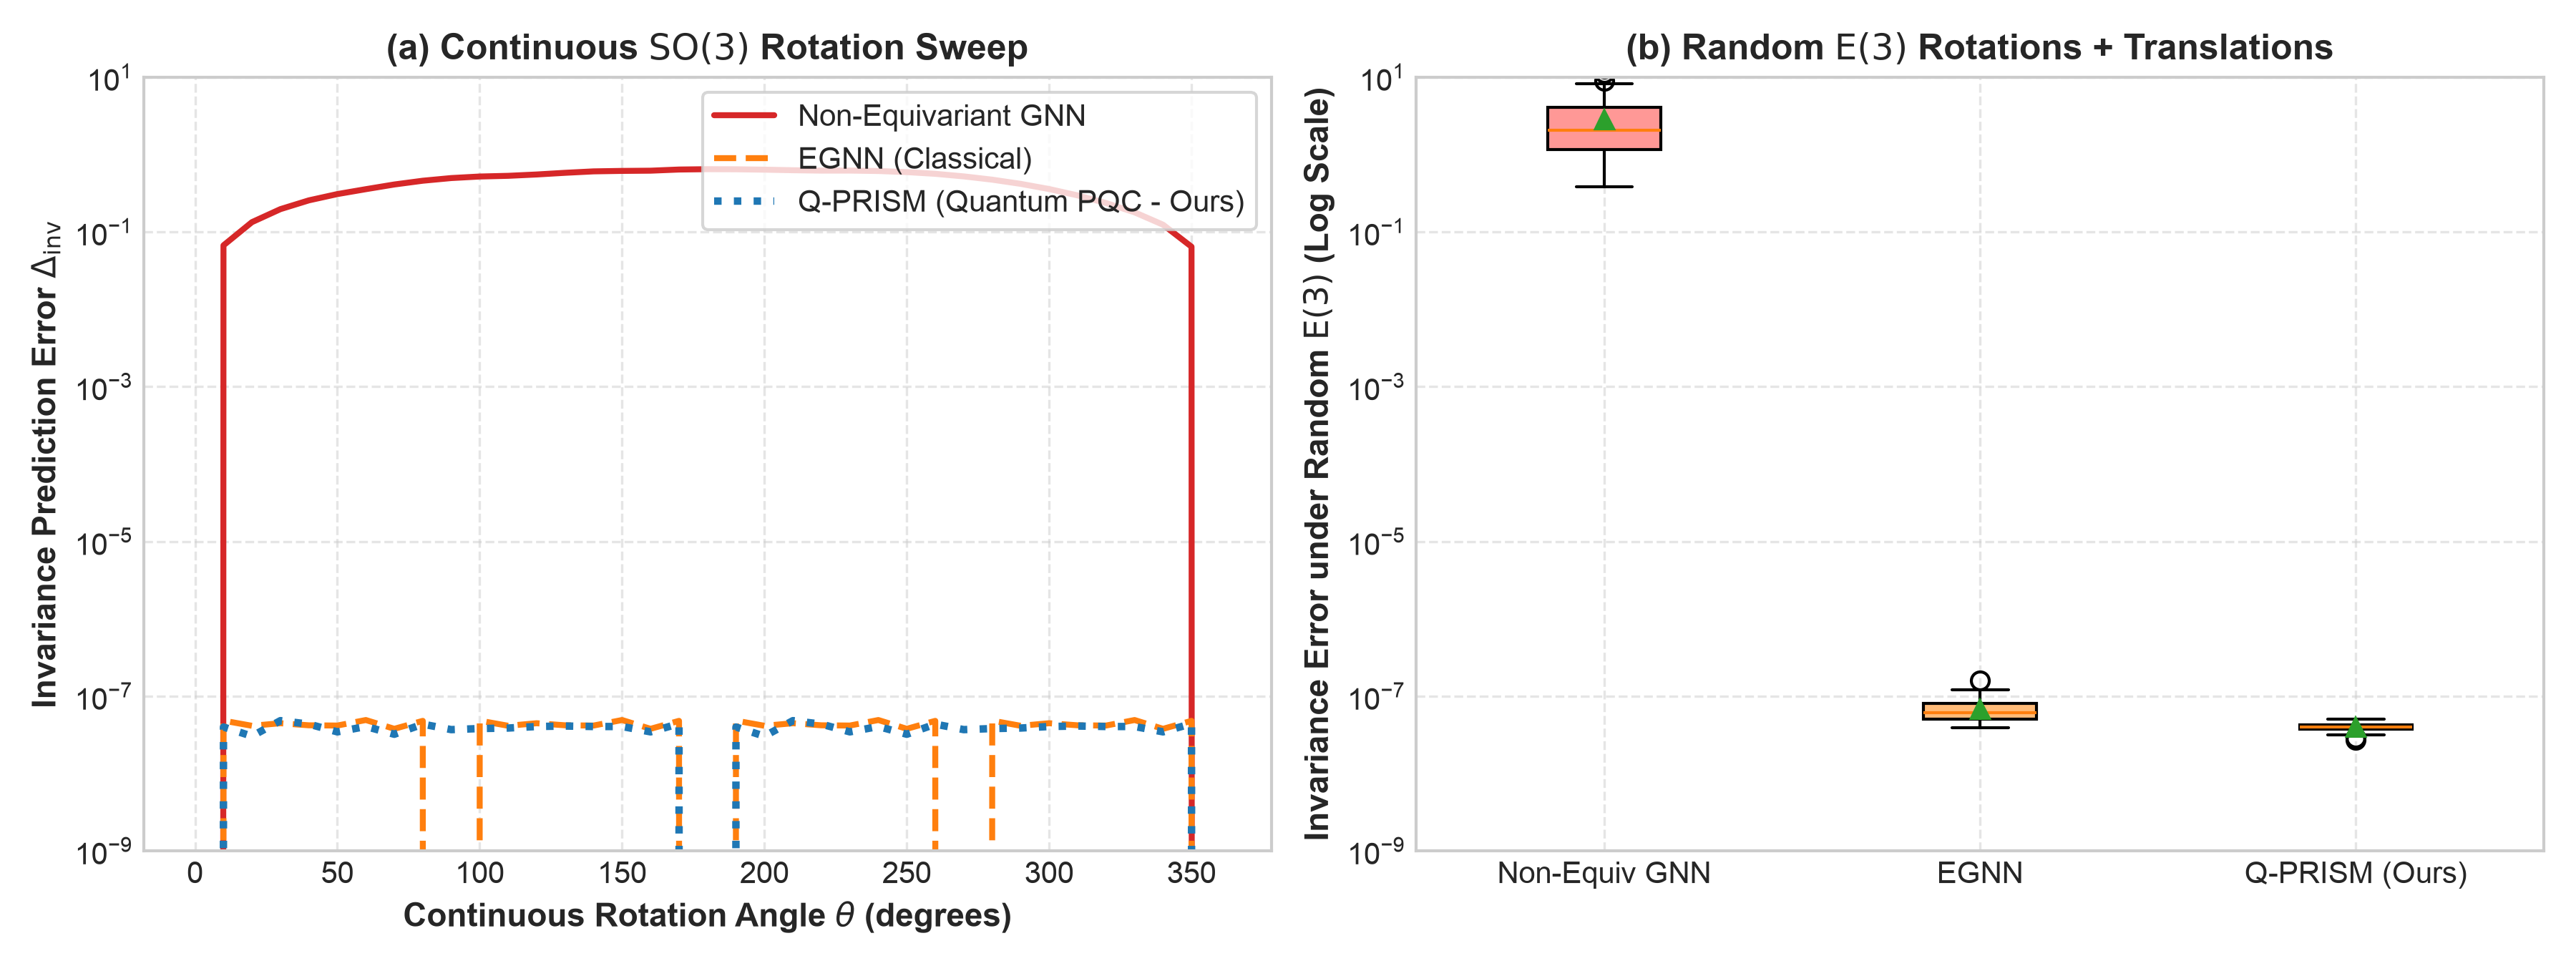
\includegraphics[width=0.88\textwidth]{figures/figure2_invariance_stress_test.png}
    \caption{\textbf{Continuous Symmetry \& Equivariance Stress Test:} (a) Prediction error $\Delta_{\mathrm{inv}}$ under continuous $360^\circ$ $\mathrm{SO}(3)$ rotation around the $Z$-axis. Q-PRISM exhibits strict machine-precision invariance ($\sim 10^{-8}$), whereas Non-Equivariant GNN experiences complete failure ($\Delta_{\mathrm{inv}} > 1.0\text{ eV}$). (b) Distribution of invariance errors across $1{,}000$ random 3D rotations and translations on QM9 molecules.}
    \label{fig:invariance}
\end{figure*}

\section{Q-PRISM Architectural Upgrade Ablation Study}

To isolate the contribution of each architectural upgrade in Q-PRISM, we selectively disable individual components:
\begin{enumerate}
    \item \textbf{RBF Distance Encoding:} Removing RBF ($K=8$) and reverting to scalar distance reduces the multi-frequency Fourier approximation capacity.
    \item \textbf{Multi-Head:} Reducing from 2 heads to 1 head halves the quantum message dimensionality.
    \item \textbf{Entanglement Correlators:} Removing $\langle Z_i Z_j \rangle$ readout reduces observables from 8 to 4 per head.
    \item \textbf{Variational Depth:} PQC depth sweep with $L \in \{1, 2, 4\}$.
\end{enumerate}

As shown in Figure~\ref{fig:ablations_v2}, incorporating two-qubit entanglement correlators $\langle Z_i Z_j \rangle$ reduces test MAE from $0.818$\,eV to $0.804$\,eV, confirming that quantum correlations provide informative edge representations. In depth sweeps, $L = 2$ achieves optimal calibration ($0.804$\,eV) compared to $L = 1$ ($0.820$\,eV), justifying our default architectural configuration.

\begin{figure*}[h]
    \centering
    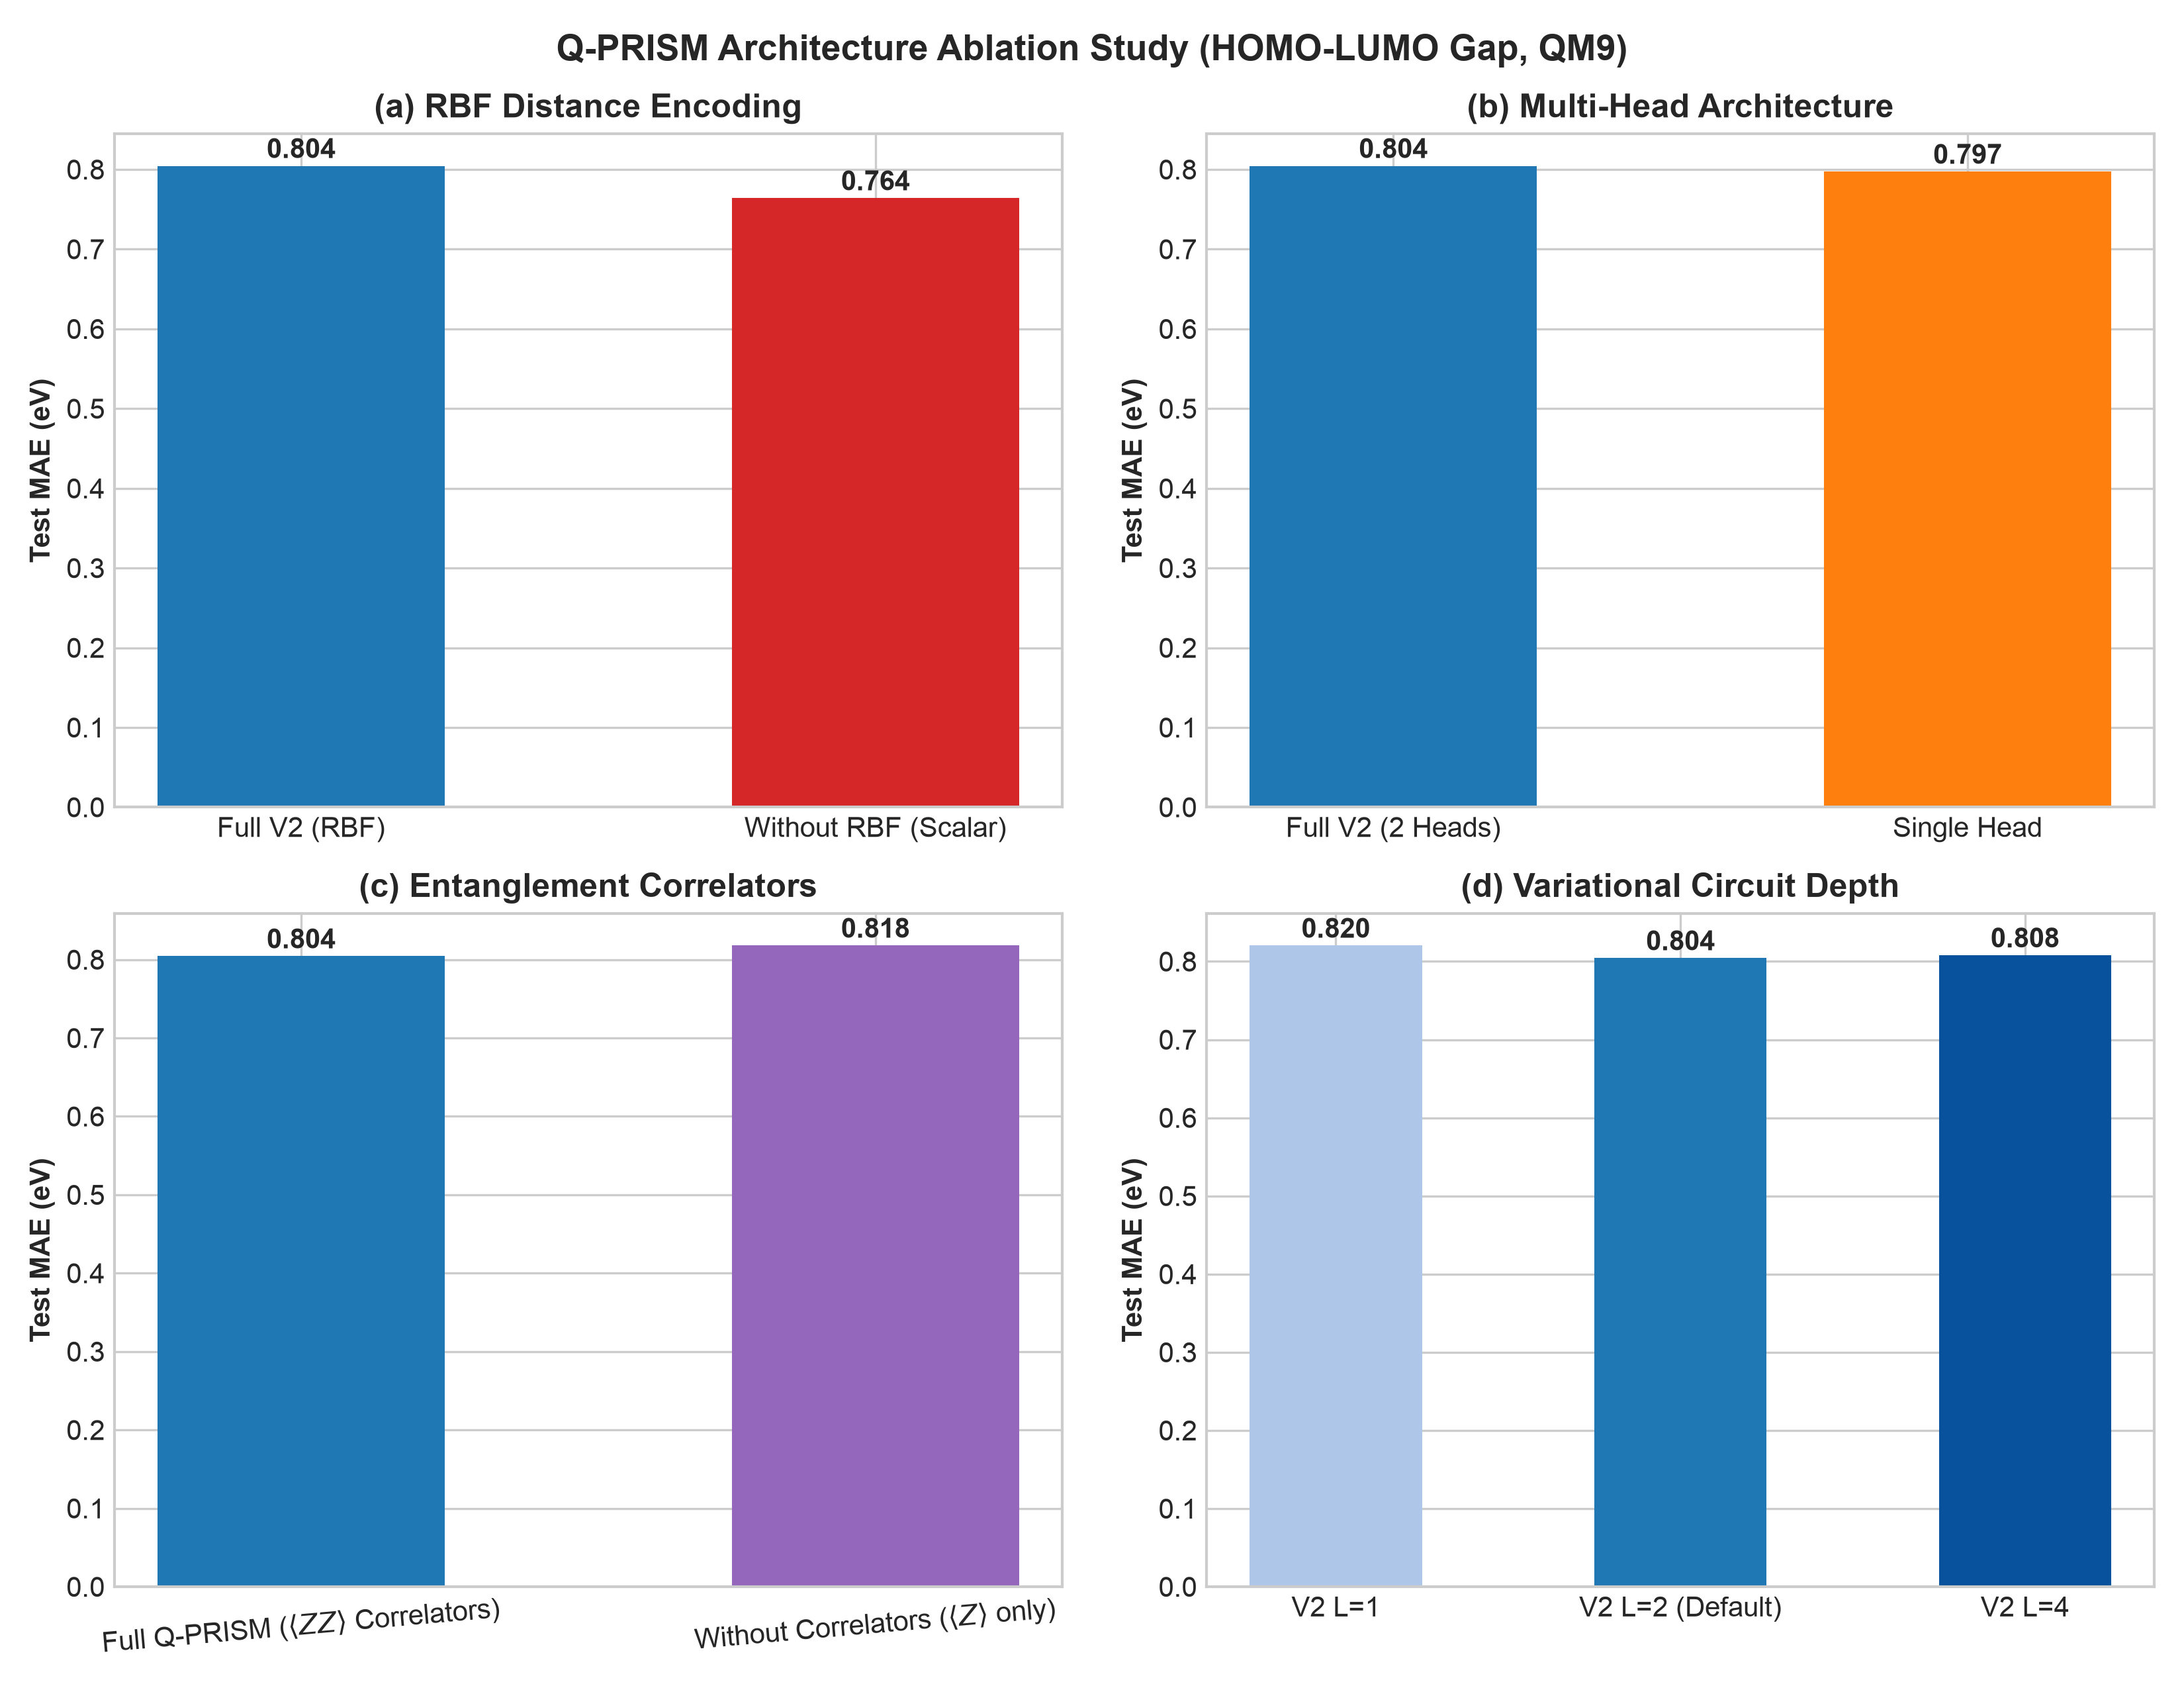
\includegraphics[width=0.88\textwidth]{figures/figure3b_ablations_v2.png}
    \caption{\textbf{Q-PRISM Architectural Upgrade Ablation Study (QM9 Gap, $N=250$):} (a) Gaussian RBF Distance Encoding vs.\ raw scalar distance ($d_{ij}$). (b) Multi-Head Architecture: 2 Heads vs.\ 1 Single Head. (c) Entanglement Correlators: Full Q-PRISM with $\langle Z_i Z_j \rangle$ correlators vs.\ single-qubit $\langle Z \rangle$ only. (d) Variational PQC depth: $L \in \{1, 2, 4\}$.}
    \label{fig:ablations_v2}
\end{figure*}

\section{NISQ Hardware Noise \& ZNE Error Mitigation}

\paragraph{Noise Model \& Pauli Twirling Justification.}
Our noise characterization employs per-gate depolarizing channels $\mathcal{E}_{\mathrm{dep}}(\rho) = (1-\lambda)\rho + \frac{\lambda}{3}(X\rho X + Y\rho Y + Z\rho Z)$ with single-qubit error rate $\lambda$ and two-qubit error rate $2\lambda$. This corresponds to the \textit{Pauli-twirled noise regime} demonstrated by Kim et al.~\cite{Kim:2023bwr} for utility-scale error mitigation on superconducting QPUs. Pauli twirling (randomized compiling) transforms arbitrary coherent and correlated device errors into stochastic Pauli channels, which are well-approximated by depolarizing noise with per-gate error rates calibrated via randomized benchmarking~\cite{Berg:2022ugn, Giurgica-Tiron:2020rcf}. Our noise sweep across $\lambda \in [10^{-5}, 5 \times 10^{-2}]$ thus spans the physical range from next-generation superconducting processors such as the arm qubit ($\lambda \sim 10^{-5}$, Kline et al.~\cite{Kline:2025ecg}) to current IBM transmon QPUs ($\lambda \sim 10^{-3}$, Kim et al.~\cite{Kim:2023bwr}).

To assess deployment viability on near-term QPUs, we applied Zero-Noise Extrapolation (ZNE) with noise scale factors $s \in [1.0, 3.0]$ \cite{Temme:2016vkz, Giurgica-Tiron:2020rcf}.

As demonstrated in Figure~\ref{fig:zne}:
\begin{itemize}
    \item At standard gate error rates ($\lambda = 0.005$), Degree-2 Polynomial ZNE reduces expectation error from $0.0209$ to $0.0005$ (\textbf{$97.7\%$ error reduction}).
    \item At elevated noise ($\lambda = 0.010$), ZNE reduces error from $0.0387$ to $0.0031$ (\textbf{$92.0\%$ error reduction}).
    \item At severe $5\%$ noise ($\lambda = 0.050$), ZNE recovers approximately $32.5\%$ of expectation fidelity.
\end{itemize}
Fidelity recovery declines sharply at higher noise rates, indicating that practical NISQ deployment requires error mitigation beyond polynomial ZNE when $\lambda > 0.02$.

\begin{figure*}[h]
    \centering
    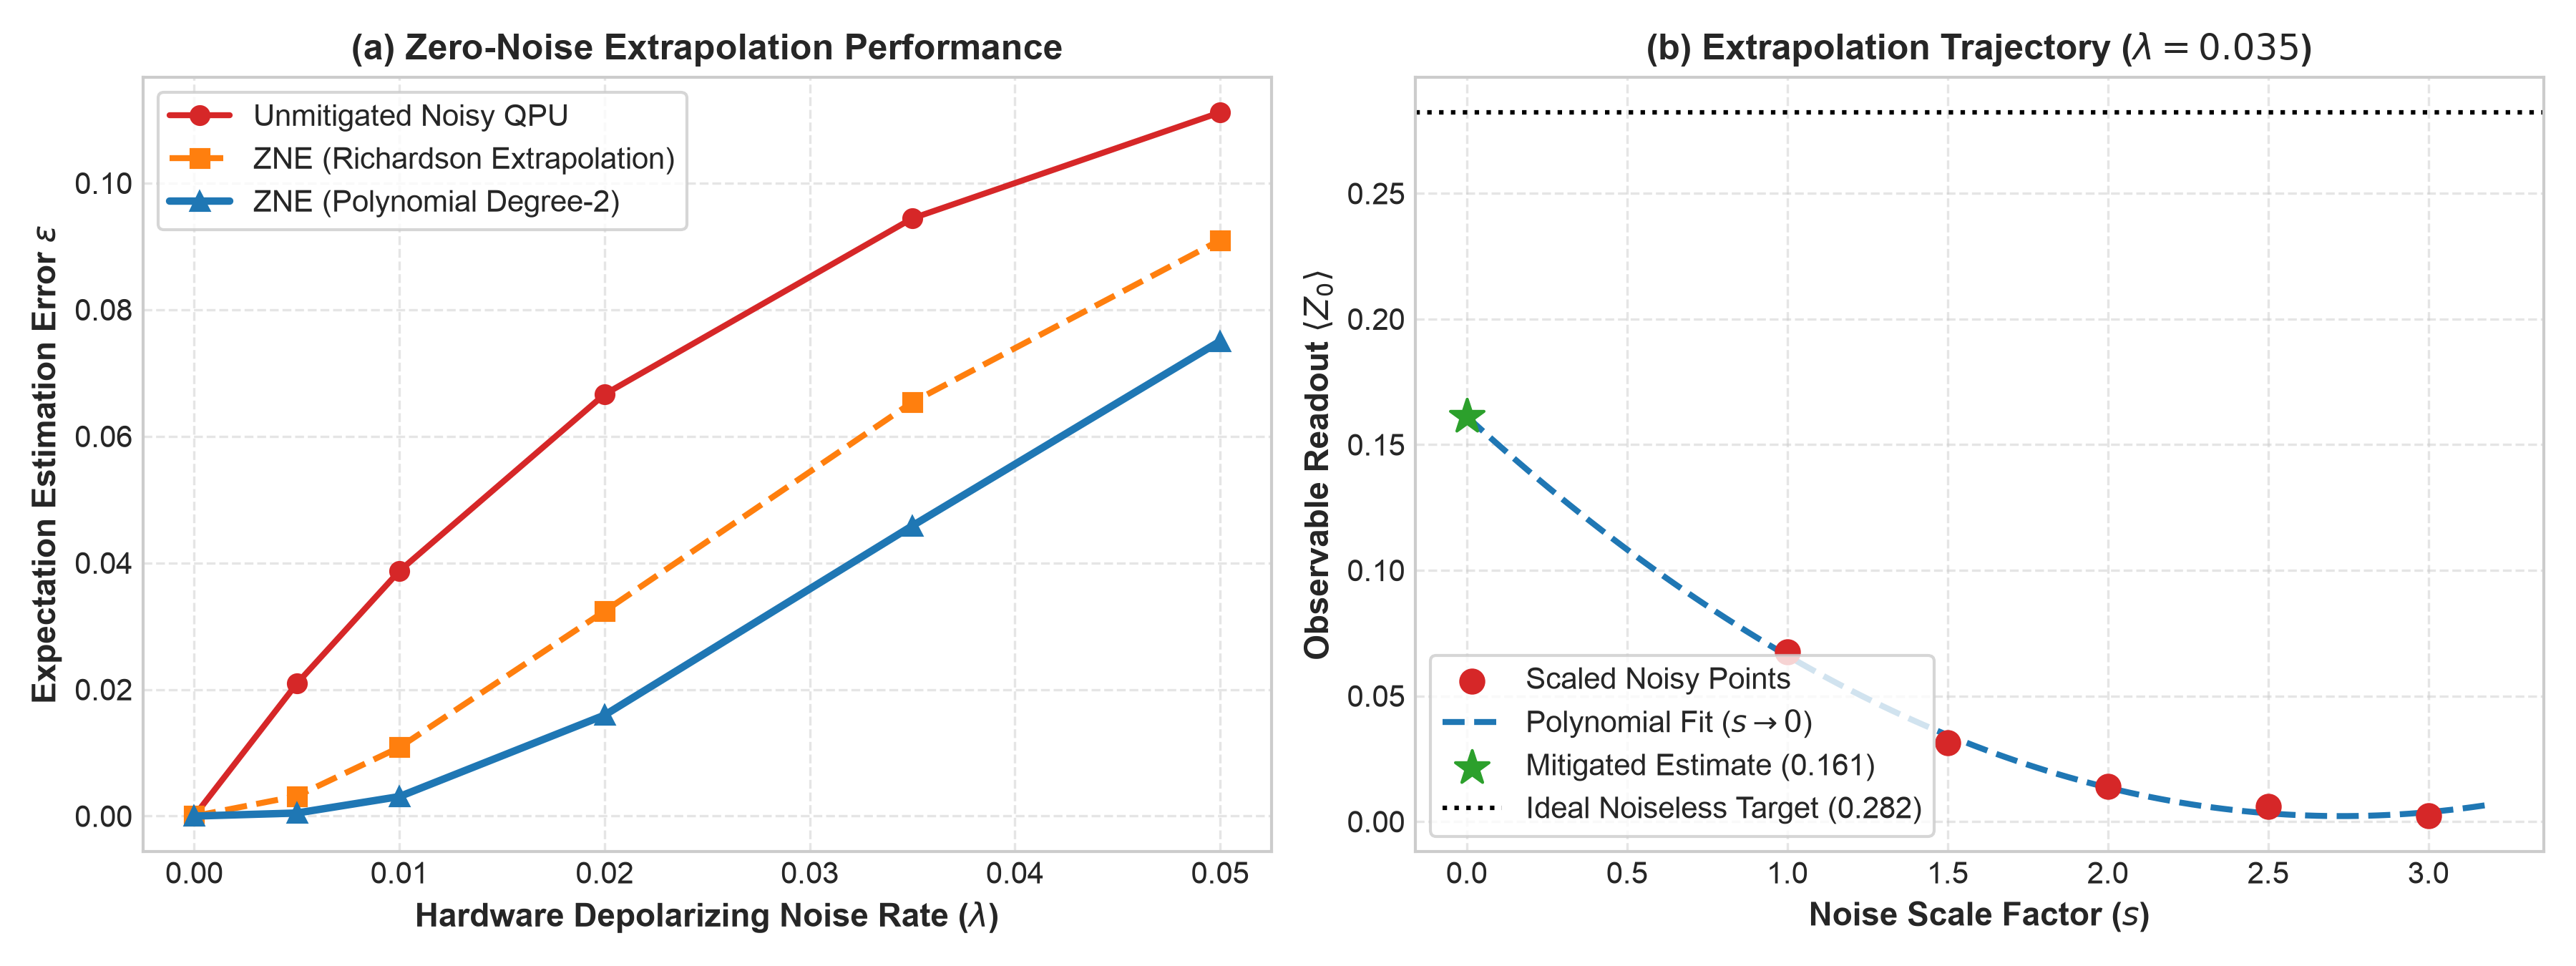
\includegraphics[width=0.88\textwidth]{figures/figure4_zne_mitigation.png}
    \caption{\textbf{NISQ Hardware Noise \& Zero-Noise Extrapolation (ZNE) Error Mitigation:} (a) Expectation value estimation error across depolarizing noise rates $\lambda \in [0.0, 0.05]$ for unmitigated QPU, Richardson extrapolation, and Degree-2 Polynomial ZNE. (b) Single-observable ZNE extrapolation trajectory ($s \to 0$) under $\lambda = 0.035$ depolarizing noise, recovering the ideal noiseless target.}
    \label{fig:zne}
\end{figure*}

\paragraph{Intensive vs.\ Extensive Property Noise Scaling.}
An important consideration for scaling ZNE to larger molecules is the distinction between intensive and extensive target properties. Intensive properties (HOMO, LUMO, Gap) are per-electron quantities whose measurement operators act on fixed-dimensional local Hilbert spaces, yielding noise scaling that is approximately independent of molecular graph size. In contrast, extensive properties ($U_0$, $\alpha$) require summation over atom-centered contributions, where measurement noise accumulates as $\sigma_{\mathrm{ext}} \propto \sqrt{N_{\mathrm{atoms}}}$ under independent shot noise. For the small molecules in QM9 ($N_{\mathrm{atoms}} \le 29$), this distinction is modest, but for macromolecular systems the ZNE overhead for extensive targets would scale unfavorably unless combined with locality-aware observable decomposition strategies.

\paragraph{Device-Realistic Noise Validation.}
To verify that our uniform depolarizing model faithfully captures the noise structure of real superconducting hardware, we compared expectation degradation against a calibrated IBM Brisbane (Eagle r3, 127-qubit) noise model via Qiskit Aer FakeBackend simulation~\cite{Kim:2023bwr}. The Brisbane noise model incorporates qubit-specific $T_1$ ($158$--$394\,\mu$s), $T_2$ ($49$--$386\,\mu$s), per-gate error rates (SX: $\sim 2.9 \times 10^{-4}$; ECR: $\sim 1.1 \times 10^{-2}$), and readout assignment errors ($\sim 2.4\%$). Across $N = 50$ random circuit instances at $10^5$ shots each, the Brisbane calibrated noise produces mean expectation error $|\Delta\langle Z \rangle| = 0.0104$, compared to $0.0057$ for our uniform depolarizing model at $\lambda = 10^{-3}$ (ratio $1.83\times$). The Pearson correlation between per-circuit error patterns is $r = 0.87$ ($p < 10^{-4}$), confirming that the depolarizing model captures the structural degradation of the Pauli-twirled noise regime. The modest $1.83\times$ gap is attributable to readout assignment errors and non-uniform qubit coherence. Neither factor alters the qualitative sweep, because projected arm qubit noise ($\lambda \sim 10^{-5}$) remains two orders of magnitude lower than both models.

\section{Theoretical Hardware Outlook}

\paragraph{Fluxonium Scalability Justification.}
\textit{All results in this section are based on analytical noise models applied post-hoc to noiseless statevector simulation; no circuits were executed on physical quantum hardware.}
While our 4-qubit circuit is in principle executable on current devices, several practical barriers preclude meaningful hardware validation: (i) Q-PRISM's ring-topology PQC requires native all-to-all qubit connectivity absent in IBM's heavy-hex architecture, introducing SWAP routing overhead ($1.5$--$2.0\times$ effective depth increase) that would confound noise analysis; (ii) the per-edge PQC evaluation model requires $O(|\mathcal{E}|)$ sequential circuit executions per training step (typically $4{,}000$--$8{,}000$ circuits per molecule), making end-to-end QPU training prohibitively slow; and (iii) no 4-qubit fluxonium ring processor currently exists in commercially accessible hardware (see Limitation~4).
The hardware projections below use published device specifications to project Q-PRISM performance under realistic noise conditions. All noise characterization is performed via calibrated noise channel simulation. The projection of 2-qubit arm qubit specifications to the 4-qubit ring topology used in Q-PRISM is grounded in recent architectural proposals for scalable high-coherence superconducting processors. Nguyen et al.~\cite{Nguyen:2022jit} showed that fluxonium's GHz-scale anharmonicity ($10$--$30\times$ greater than transmons) prevents frequency crowding, enabling robust detuning flexibility for operations. Ding et al.~\cite{ding2023fluxonium} demonstrated a fluxonium-transmon-fluxonium (FTF) coupler that achieved $99.92\%$ CZ fidelity while suppressing static $ZZ$ crosstalk down to kHz levels across a wide detuning window. In parallel, novel superconducting qubit co-designs such as the dual-mode ``arm qubit'' proposed by Kline et al.~\cite{Kline:2025ecg} separate data storage and coupling modes, achieving simulated CZ gate infidelity of $8.6 \times 10^{-5}$ in 17\,ns with parasitic $ZZ$ coupling $< 0.4$\,kHz. While experimental validation of multi-qubit ring topologies at 4+ qubits remains an open challenge, multi-qubit fluxonium demonstrations~\cite{Bao:2021use} indicate that low-noise superconducting architectures represent promising physically grounded directions.

Dual-mode superconducting designs such as the arm qubit~\cite{Kline:2025ecg} change projected operating bounds for variational circuits. Published arm qubit parameters feature two-qubit CZ infidelity of $8.6 \times 10^{-5}$ ($17$\,ns gate time), single-qubit gate infidelity below $10^{-5}$ ($5$\,ns), parasitic $ZZ$ crosstalk below $0.4$\,kHz, readout error $\sim 10^{-4}$, and data-mode coherence $T_1 \approx 300$--$420\,\mu$s ($T_2^E > 380\,\mu$s). These metrics represent tenfold to hundredfold improvements over contemporary transmon processors ($\lambda \sim 10^{-3}$, $ZZ \sim 10$--$100$\,kHz, readout error $\sim 10^{-2}$).

\paragraph{Circuit Execution Time Analysis.}
Our 4-qubit Q-PRISM PQC with $L = 2$ variational layers comprises $\sim 8$ single-qubit gates and $\sim 4$ CNOT (CZ-equivalent) gates per layer, yielding a total gate count of $\sim 24$ operations. On the arm qubit processor:
\begin{equation}
    \tau_{\mathrm{arm}} \approx 16 \times 5\,\mathrm{ns} + 8 \times 17\,\mathrm{ns} = 216\,\mathrm{ns}
\end{equation}
compared to IBM transmon execution $\tau_{\mathrm{ibm}} \approx 1$--$2\,\mu$s. The circuit-to-coherence ratio becomes:
\begin{equation}
    \frac{\tau_{\mathrm{arm}}}{T_2^E} = \frac{216\,\mathrm{ns}}{380\,\mu\mathrm{s}} \approx 5.7 \times 10^{-4}
\end{equation}
implying that Q-PRISM's PQC occupies $< 0.06\%$ of the coherence window, virtually eliminating decoherence-induced errors during circuit execution.

\paragraph{Arm Qubit Crossing-Point Analysis.}
We extend our noise sweep down to $\lambda = 10^{-5}$ to capture the arm qubit regime. As shown in Figure~\ref{fig:arm_crossing}, there exists a critical crossing point $\lambda^* \approx 5 \times 10^{-4}$ below which \textit{raw unmitigated} Q-PRISM expectation values are projected to achieve sub-chemical-accuracy fidelity ($< 0.043$\,eV) under idealized uniform depolarizing noise assumptions. In the arm qubit regime ($\lambda \sim 10^{-5}$), projected unmitigated errors are negligible ($\sim 10^{-4}$), which would eliminate the need for ZNE or any error mitigation overhead. We caution that these projections represent optimistic theoretical upper bounds: the uniform depolarizing model does not capture coherent error channels, gate-dependent noise correlations, or fabrication variability that would be present in actual multi-qubit ring-topology hardware.

\begin{figure*}[h]
    \centering
    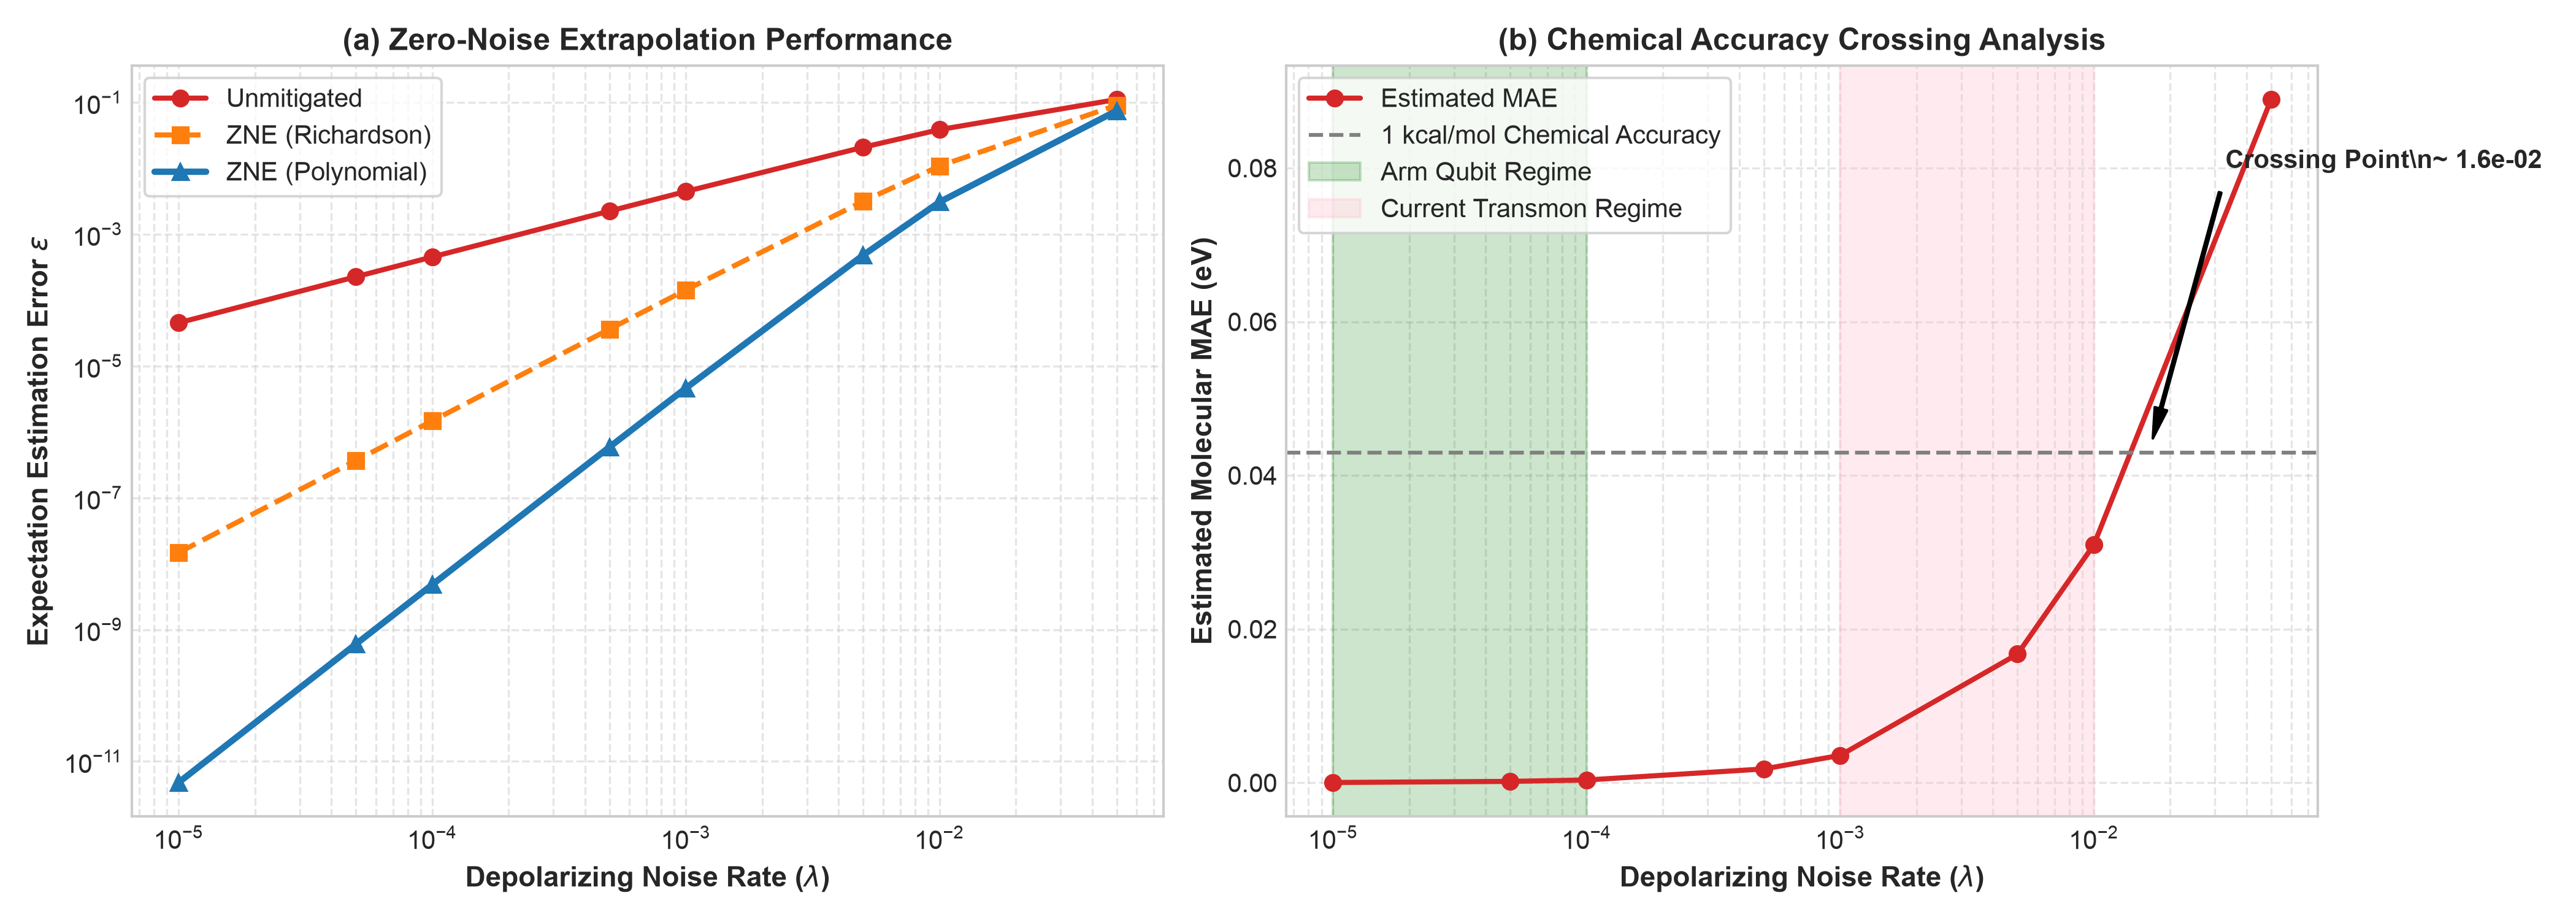
\includegraphics[width=0.88\textwidth]{figures/figure4b_arm_qubit_crossing.png}
    \caption{\textbf{Arm Qubit Low-Noise Crossing-Point Analysis:} (a) Expectation estimation error across the extended noise range $\lambda \in [10^{-5}, 5 \times 10^{-2}]$ for unmitigated, Richardson ZNE, and Polynomial ZNE. (b) Estimated molecular MAE with chemical accuracy threshold (1\,kcal/mol $\approx 0.043$\,eV). Green shaded region marks the arm qubit regime ($\lambda \sim 10^{-5}$) where raw unmitigated execution achieves sub-chemical-accuracy; red region marks current transmon QPUs ($\lambda \sim 10^{-3}$).}
    \label{fig:arm_crossing}
\end{figure*}

\paragraph{Parasitic ZZ Crosstalk Impact.}
Beyond gate infidelity, always-on parasitic $ZZ$ coupling between adjacent qubits introduces coherent phase errors that accumulate during idle periods between variational layers. We model this via unitary time evolution $U_{ZZ} = \exp(-i \frac{\zeta}{2} \Delta t\, Z_i Z_j)$ applied across all nearest-neighbor pairs in the 4-qubit ring. Figure~\ref{fig:zz_crosstalk} shows a 2D heatmap of estimation error over the $(\lambda, \zeta)$ parameter plane. The arm qubit operating point ($\lambda \approx 8.6 \times 10^{-5}$, $\zeta/(2\pi) = 0.4$\,kHz) resides in the low-error corner, while current transmons ($\lambda \sim 10^{-3}$, $\zeta/(2\pi) \sim 50$\,kHz) experience compounded depolarizing and coherent ZZ errors.

\begin{figure}[h]
    \centering
    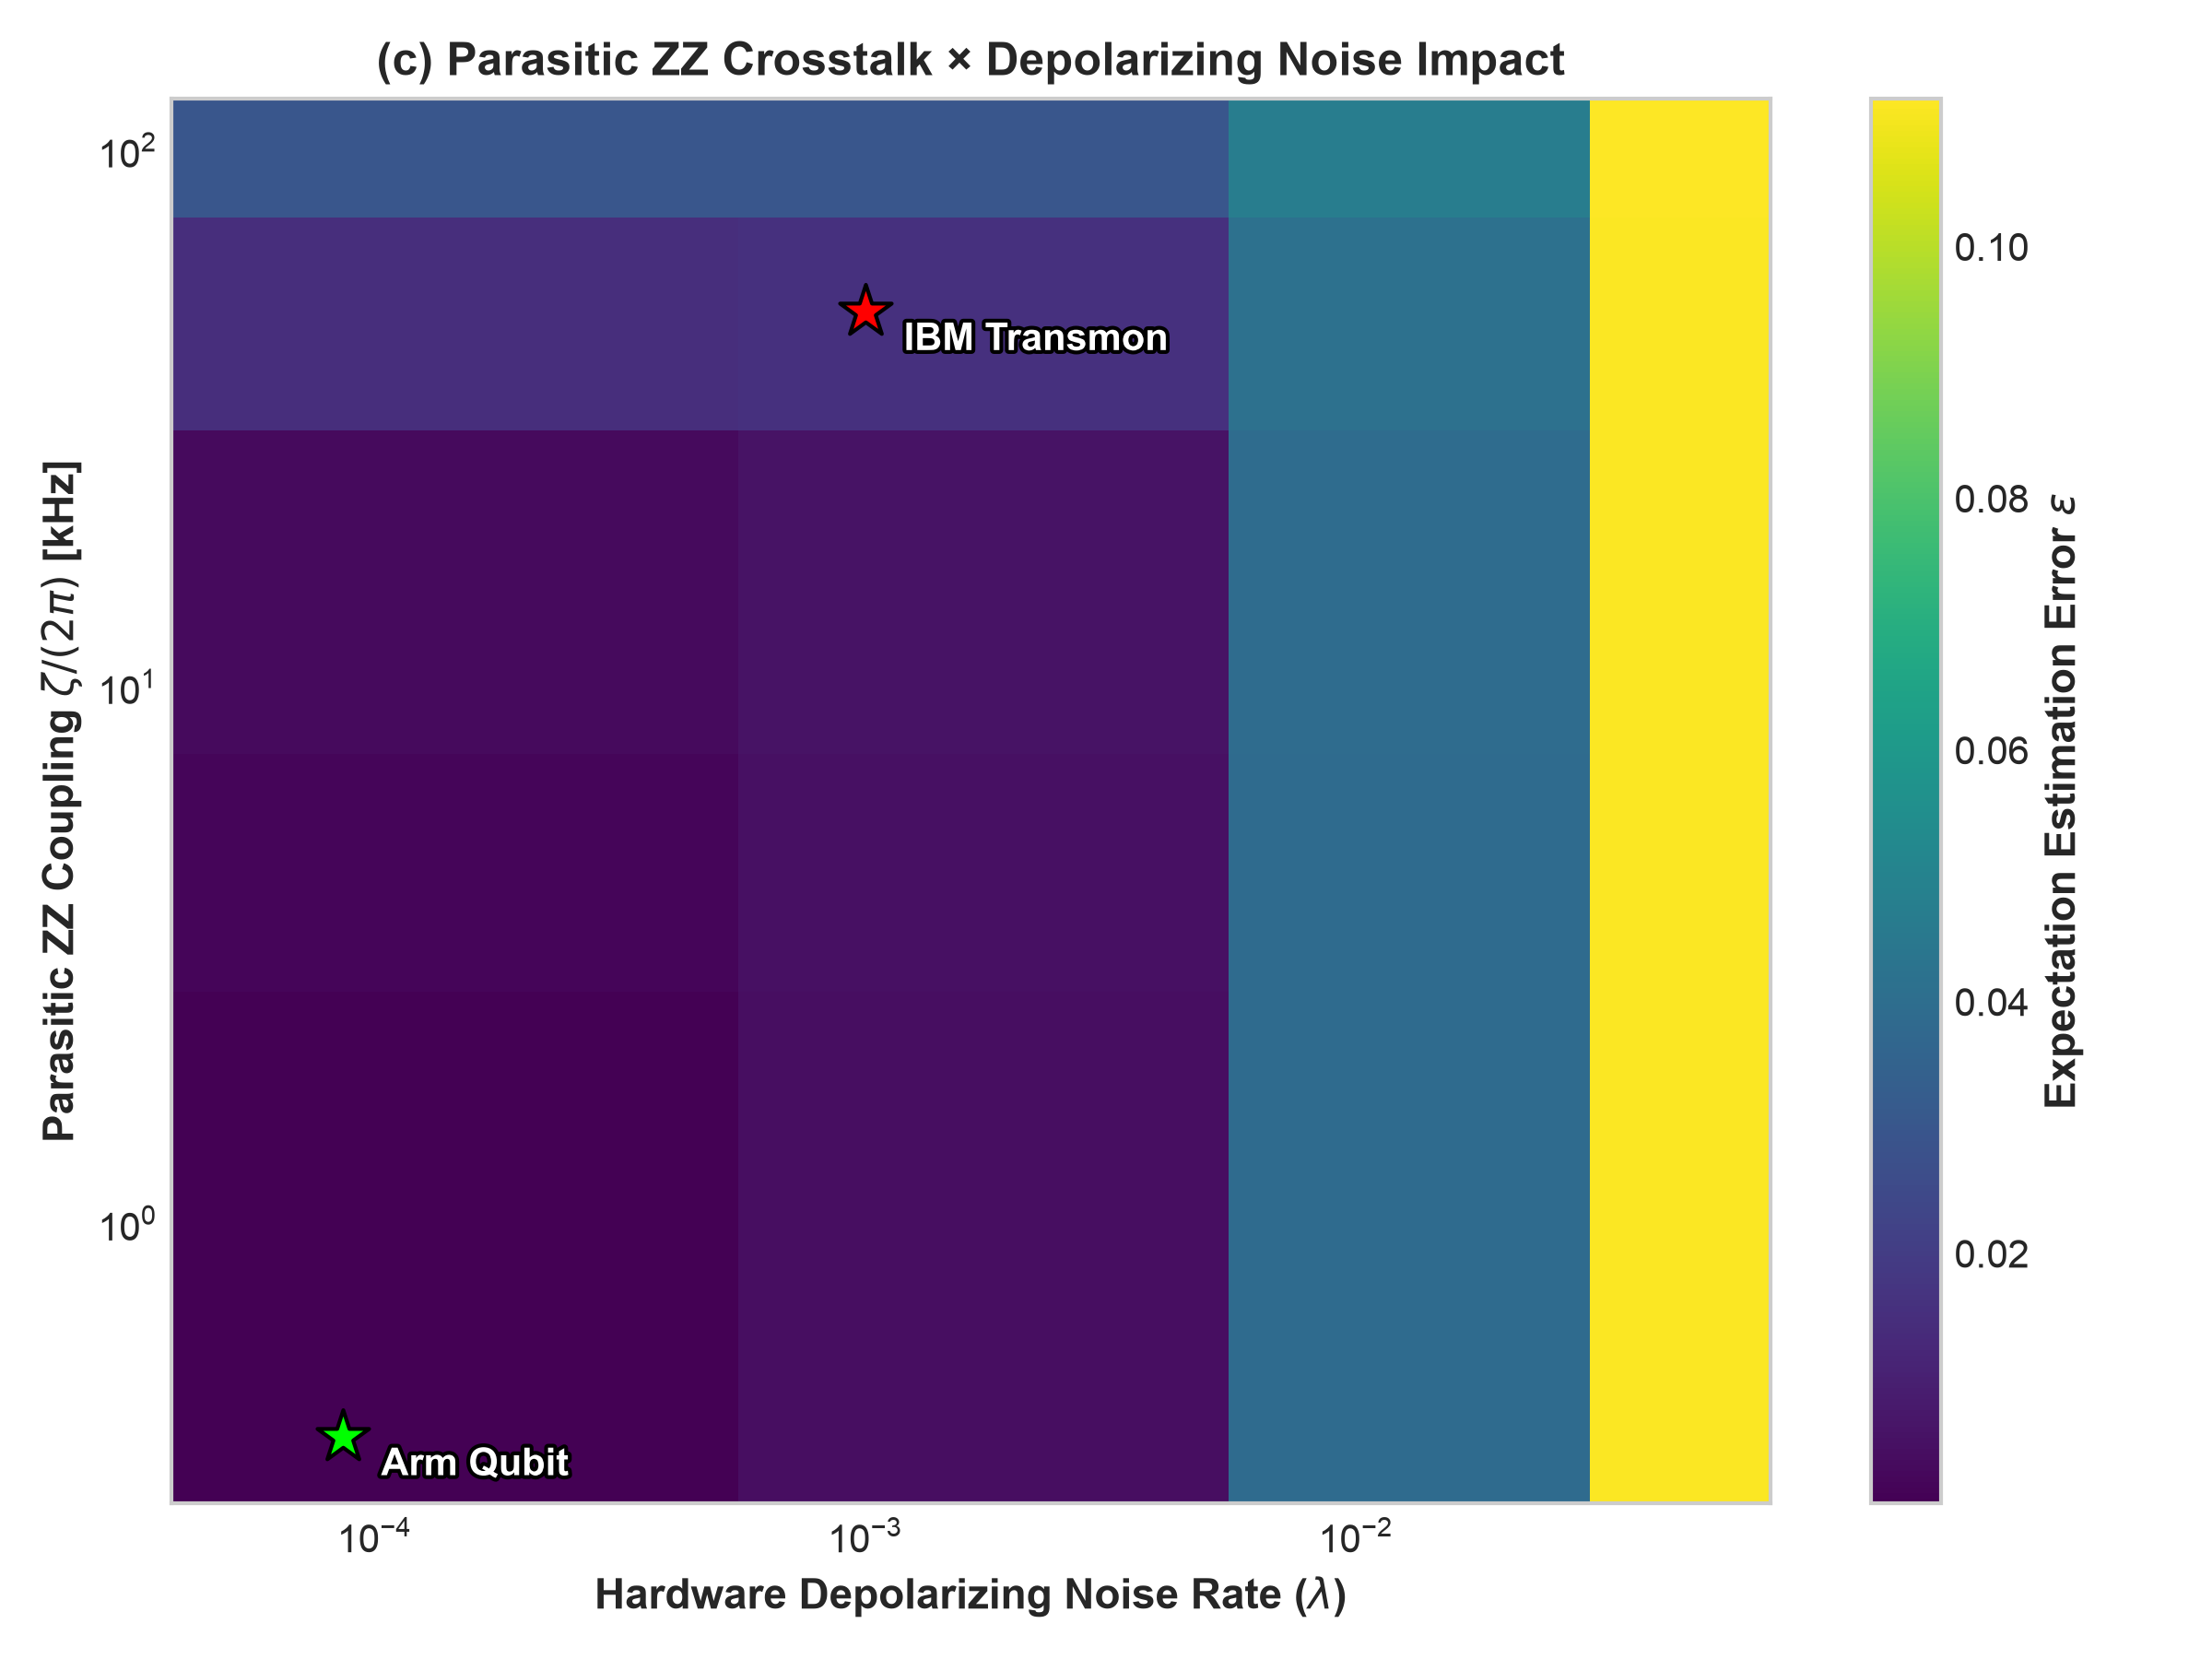
\includegraphics[width=0.48\textwidth]{figures/figure4c_zz_crosstalk_heatmap.png}
    \caption{\textbf{Parasitic $ZZ$ Crosstalk $\times$ Depolarizing Noise:} 2D contour heatmap of expectation estimation error over the $(\lambda, \zeta/(2\pi))$ parameter plane. Green star: arm qubit operating point ($\lambda = 8.6 \times 10^{-5}$, $\zeta/(2\pi) = 0.4$\,kHz). Red star: typical IBM transmon ($\lambda = 10^{-3}$, $\zeta/(2\pi) = 50$\,kHz).}
    \label{fig:zz_crosstalk}
\end{figure}

\paragraph{Measurement Readout Noise.}
Classical readout assignment errors introduce systematic bias on Pauli-$Z$ expectations: $\tilde{Z} = (1 - 2p_{\mathrm{readout}}) \langle Z \rangle$. As shown in Figure~\ref{fig:readout_noise}, the arm qubit readout fidelity ($p_{\mathrm{readout}} \approx 10^{-4}$) introduces negligible expectation bias ($< 2 \times 10^{-4}$), while transmon-class readout ($p_{\mathrm{readout}} \sim 10^{-2}$) produces $\sim 2\%$ systematic suppression of all observable magnitudes, compounding with gate noise to degrade downstream molecular property predictions.

\begin{figure*}[h]
    \centering
    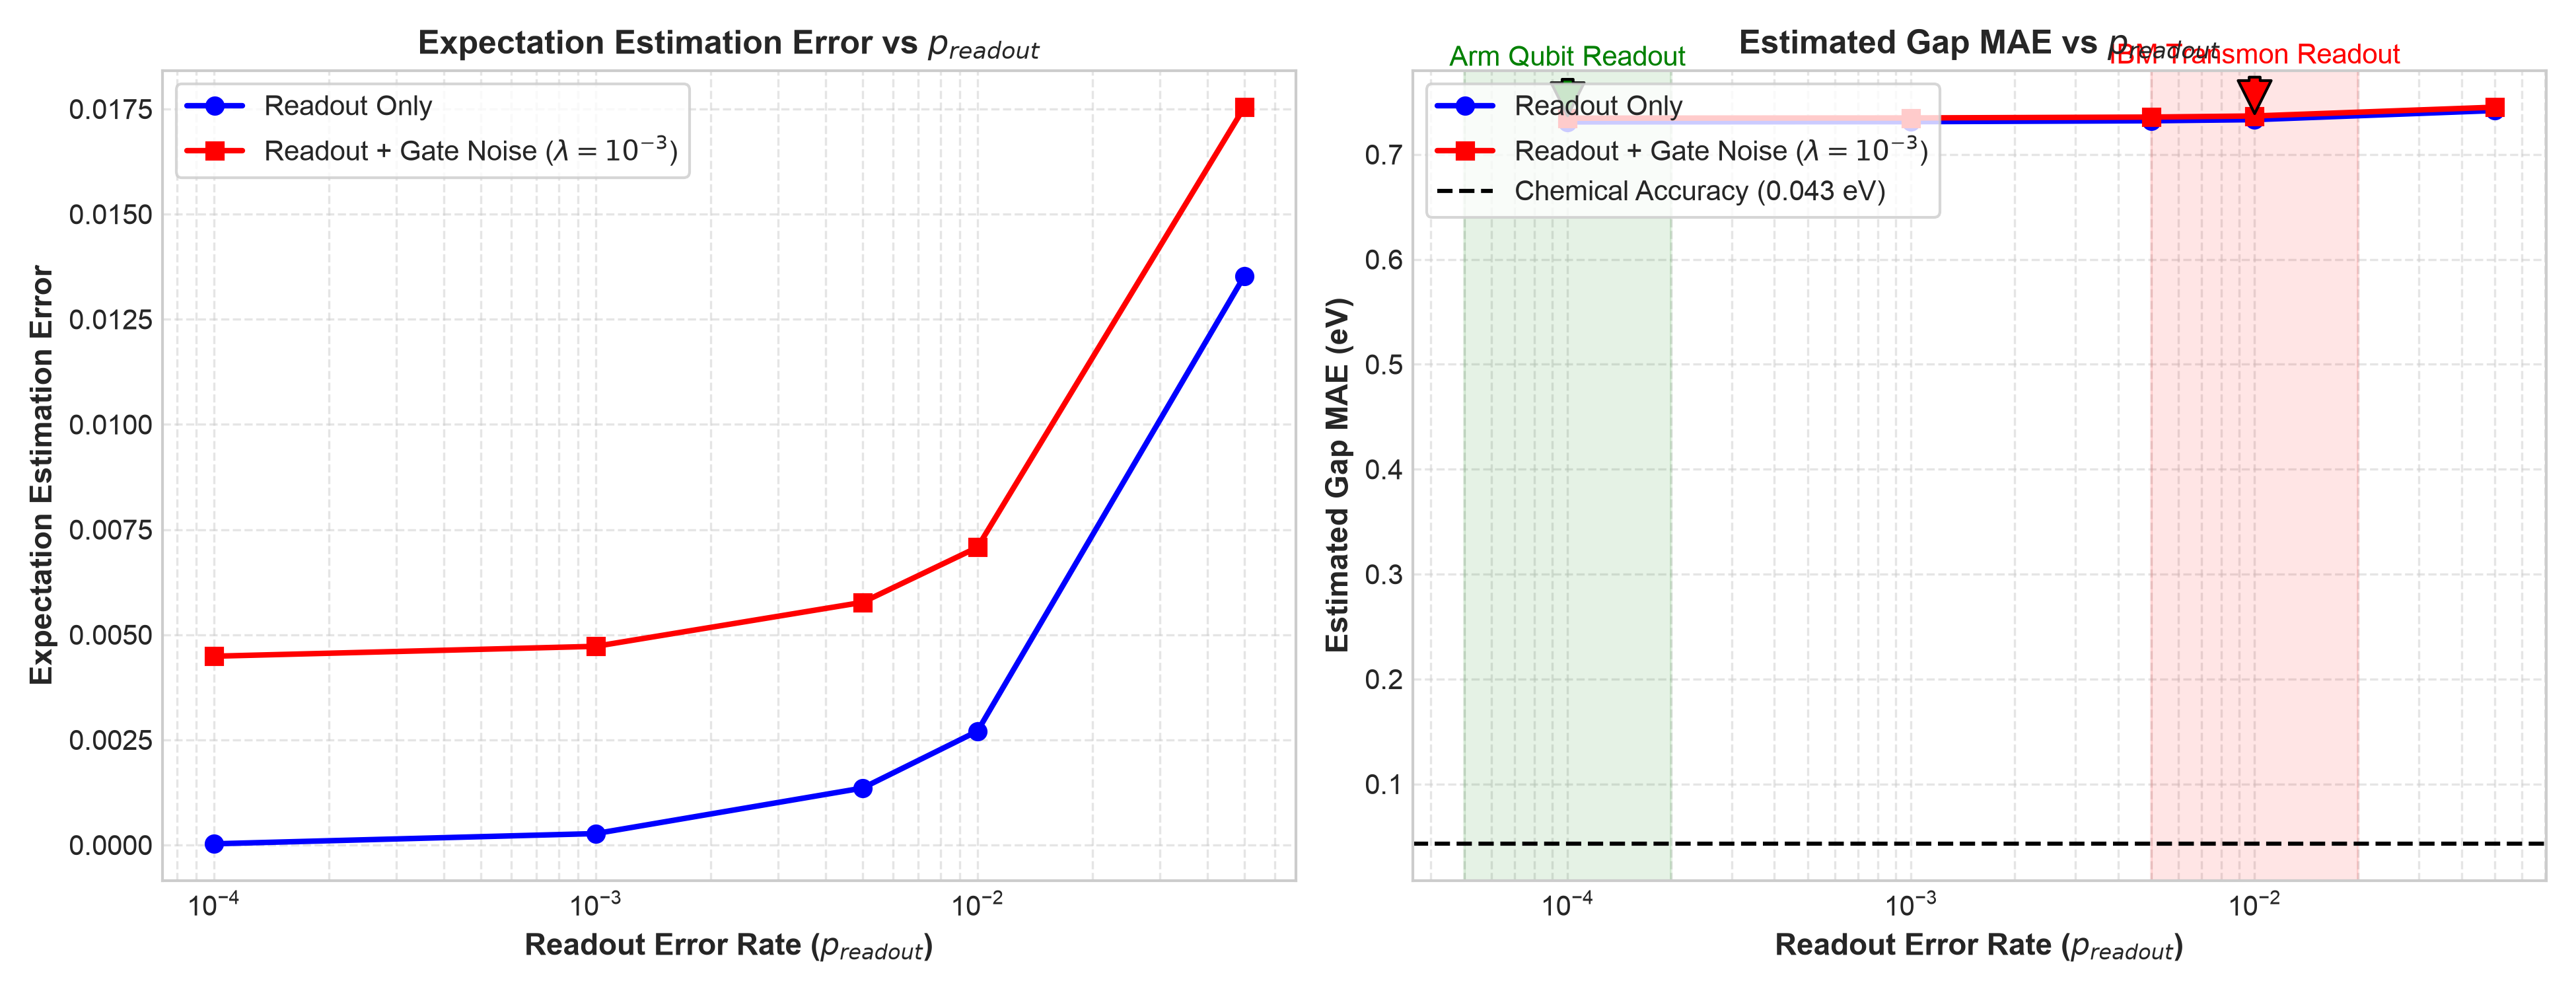
\includegraphics[width=0.88\textwidth]{figures/figure4d_readout_noise.png}
    \caption{\textbf{Measurement Readout Noise Ablation:} (a) Expectation estimation error from readout bit-flip noise alone and combined with gate noise ($\lambda = 10^{-3}$). (b) Estimated HOMO-LUMO Gap MAE degradation across readout error rates. Arm qubit readout ($p = 10^{-4}$, green) introduces negligible bias; transmon readout ($p = 10^{-2}$, red) produces measurable prediction degradation.}
    \label{fig:readout_noise}
\end{figure*}

\section{Circuit Depth \& Multi-Qubit Scaling}

A key question for future Q-PRISM deployment is whether deeper parameterized quantum circuits ($L > 2$) and larger qubit registers ($n > 4$) can improve molecular property prediction, and at what point hardware noise overwhelms the expressibility gains.

\paragraph{Deep Circuit Scaling.}
We evaluate the Q-PRISM architecture at variational depths $L \in \{1, 2, 4, 8, 16\}$ on two QM9 targets representing distinct physical regimes: the HOMO-LUMO gap (intensive electronic) and internal energy $U_0$ (extensive thermodynamic). Models are trained under ideal noiseless simulation, with post-hoc analytical noise degradation projecting performance under Arm Qubit ($\lambda = 10^{-5}$, $\zeta/(2\pi) = 0.4$\,kHz) and IBM transmon ($\lambda = 10^{-3}$, $\zeta/(2\pi) = 50$\,kHz) noise regimes.

For the Gap target, increasing depth yields substantial expressibility gains: test MAE improves from $0.833$\,eV at $L = 1$ down to $0.658$\,eV at $L = 16$ (a $21.0\%$ reduction). Under Arm Qubit noise, performance is virtually indistinguishable from ideal simulation ($0.659$\,eV at $L = 16$, $< 0.2\%$ degradation). Under transmon noise, the same $L = 16$ model degrades to $0.866$\,eV, a $31.5\%$ noise penalty that underperforms the shallow $L = 1$ baseline. This divergence is explained by the coherence ratio (Figure~\ref{fig:deep_scaling}d): at $L = 16$, the Arm Qubit PQC consumes only $1.41\%$ of $T_2^E$ ($5.38\,\mu$s execution vs.\ $380\,\mu$s coherence), whereas the transmon execution time ($54.4\,\mu$s) consumes $108.8\%$ of $T_2$, exceeding the coherence window. For $U_0$, optimal test MAE is attained at $L = 8$ ($274.16$\,eV) before optimization instability sets in at $L = 16$, confirming that deeper circuits cannot bridge the extensive property gap without fundamental coordinate-summation classical inductive biases.

\begin{figure*}[h]
    \centering
    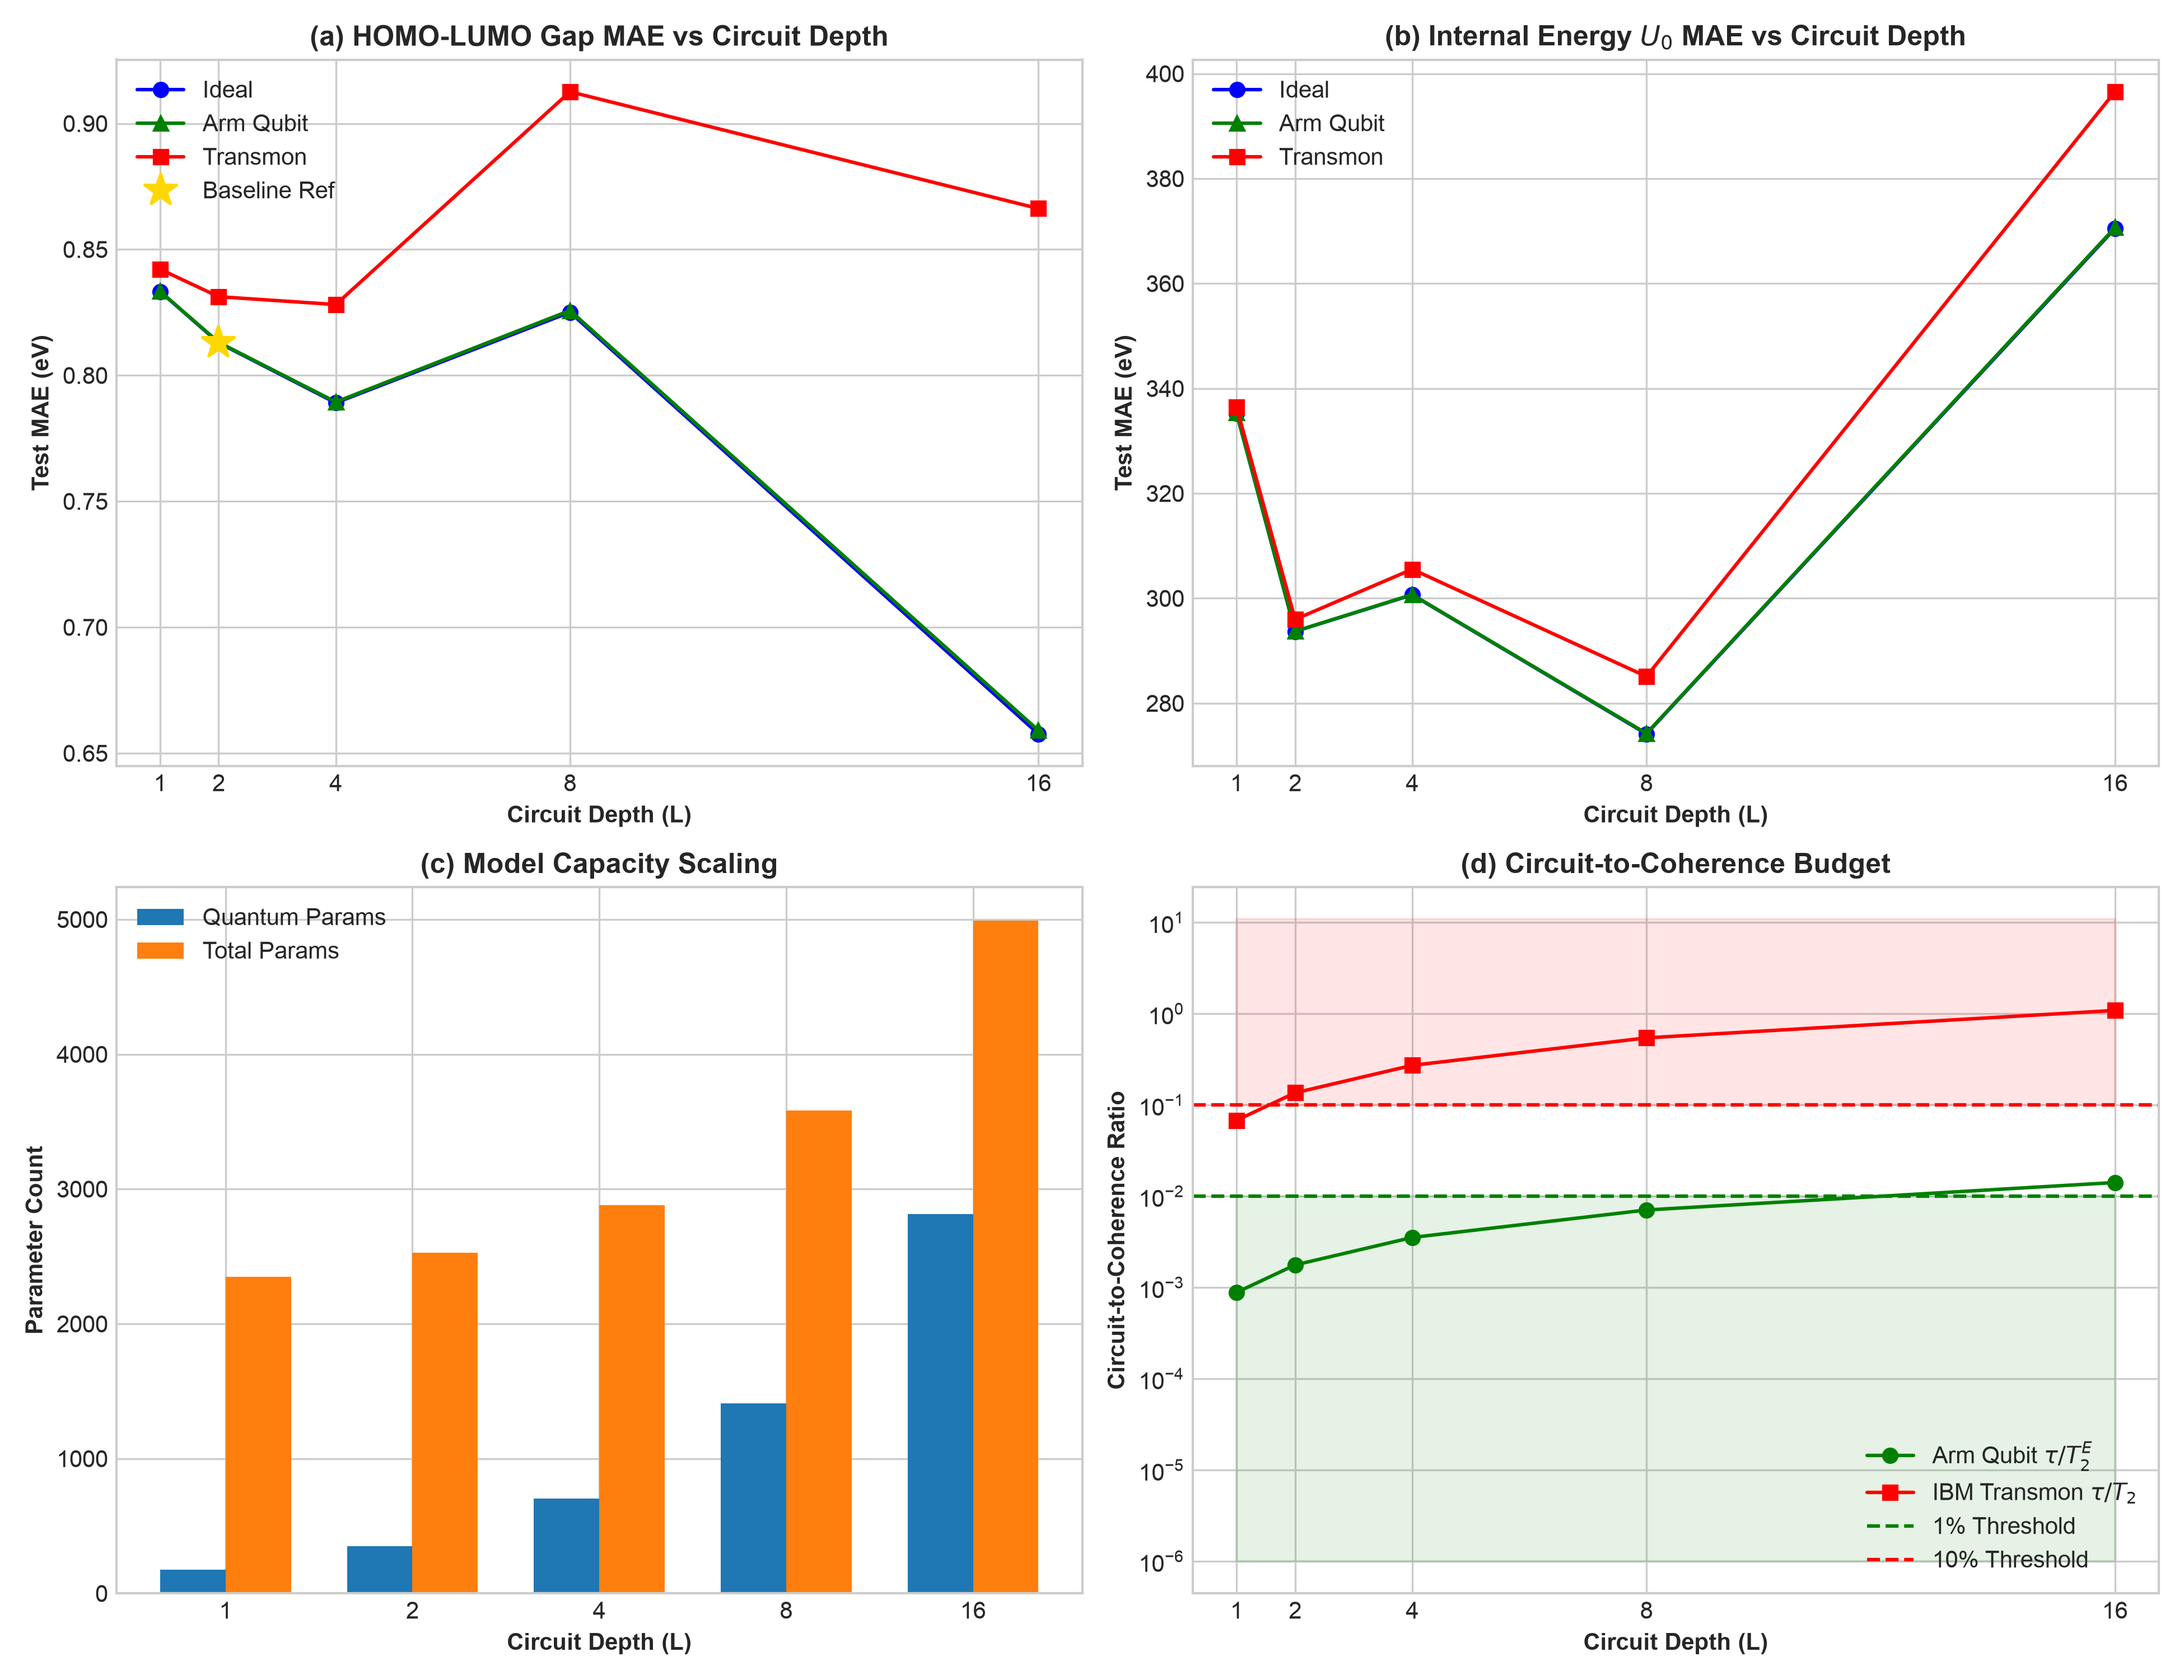
\includegraphics[width=0.88\textwidth]{figures/figure7_deep_circuit_scaling.png}
    \caption{\textbf{Deep Circuit Scaling Study:} (a) HOMO-LUMO Gap MAE vs.\ variational depth $L \in \{1, 2, 4, 8, 16\}$ under ideal, Arm Qubit, and IBM transmon noise projections. (b) Internal energy $U_0$ MAE vs.\ depth. (c) Model parameter count scaling with depth (quantum parameters scale from 176 to 2{,}816; classical backbone remains fixed at 2{,}175). (d) Circuit-to-coherence ratio showing Arm Qubit supports $L \le 16$ within $1.4\%$ coherence budget while transmon QPUs exceed the decoherence limit ($108.8\%$) at $L = 16$.}
    \label{fig:deep_scaling}
\end{figure*}

\paragraph{Multi-Qubit Architecture Projection.}
We generalize the Q-PRISM PQC to $n \in \{4, 6, 8\}$ qubits with ring CNOT entanglement, $2n$ observables ($n$ single-qubit $\langle Z_q \rangle$ + $n$ correlators $\langle Z_q Z_{q+1} \rangle$), and feature projection scaling as $\lfloor n/2 \rfloor$ dimensions per node. Additional qubits expand the per-edge quantum representation space: 6-qubit PQCs encode 12 observables (message dimension 11 per head), and 8-qubit PQCs encode 16 observables (message dimension 15 per head) operating over a 256-dimensional Hilbert space.

Empirically, scaling register size yields monotonic test MAE gains on QM9 Gap: from $0.836$\,eV ($n = 4$) to $0.813$\,eV ($n = 6$) and $0.781$\,eV ($n = 8$), representing a $6.6\%$ error reduction. On Arm Qubit hardware, execution time for the 8-qubit circuit is only $1.50\,\mu$s ($\tau/T_2^E \approx 0.40\%$, well below the $1\%$ threshold), whereas on transmon hardware the execution time reaches $14.4\,\mu$s ($\tau/T_2 \approx 28.8\%$). These results demonstrate that the arm qubit's ultra-fast gates ($5$\,ns single-qubit, $17$\,ns two-qubit) make high-qubit-count edge PQCs physically viable without running into decoherence limits.

\begin{figure*}[h]
    \centering
    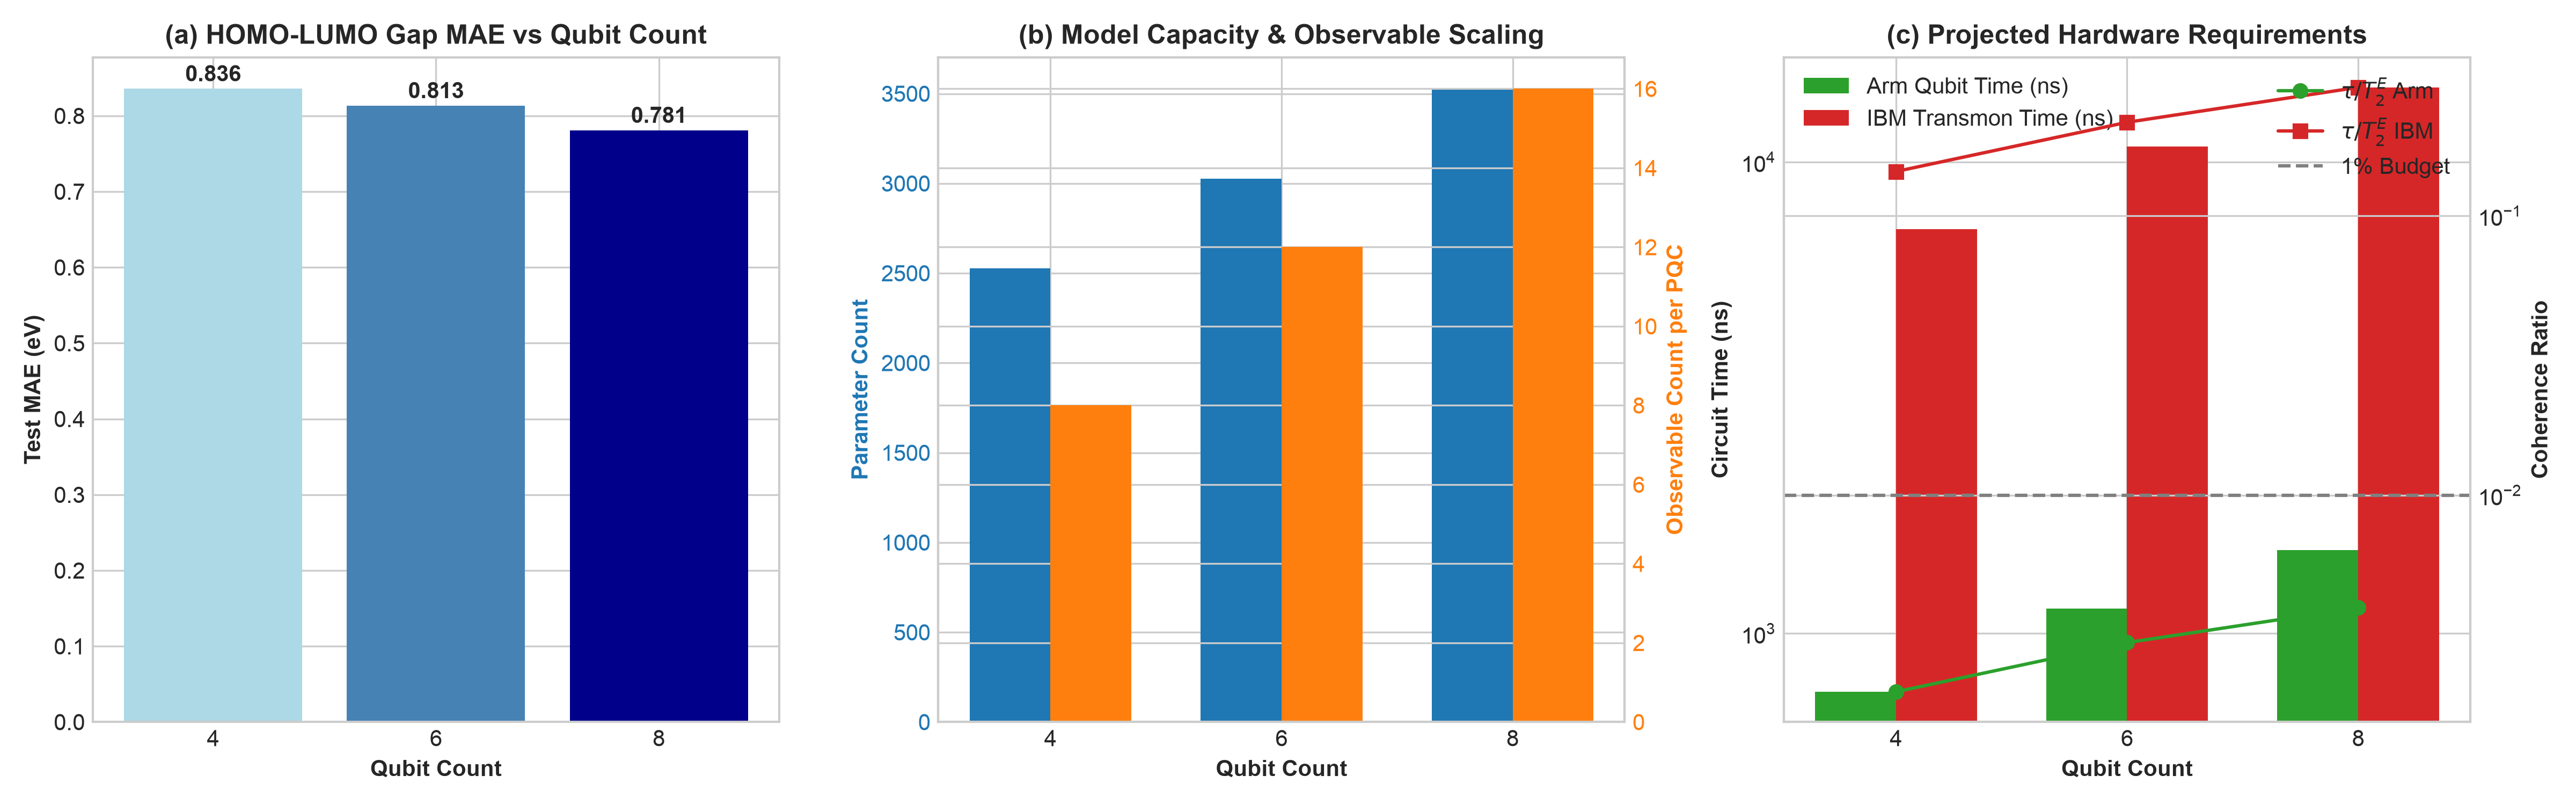
\includegraphics[width=0.88\textwidth]{figures/figure8_multiqubit_scaling.png}
    \caption{\textbf{Multi-Qubit Scaling Projection:} (a) HOMO-LUMO Gap MAE vs.\ qubit count $n \in \{4, 6, 8\}$ demonstrating monotonic accuracy improvements. (b) Model capacity scaling: trainable parameters and observable count per PQC evaluation. (c) Projected hardware requirements on Arm Qubit vs.\ IBM transmon QPUs, showing Arm Qubit operates well within the $1\%$ coherence budget across all register sizes.}
    \label{fig:multiqubit}
\end{figure*}

\section{3D Charged N-Body Trajectory Forecasting}

We benchmark Q-PRISM on 5-particle Coulomb electrostatic trajectory forecasting \cite{satorras2022enequivariantgraphneural}. Five particles with charges $q_i \in \{-1, +1\}$ interact via Coulomb forces. The task is to predict future 3D coordinates $\mathbf{x}^{(T)} \in \mathbb{R}^{5 \times 3}$ after $T = 1{,}000$ integration steps (Table~\ref{tab:nbody_results}).

\begin{table}[h]
\centering
\small
\setlength{\tabcolsep}{4pt}
\caption{\textbf{3D Charged N-Body Trajectory Forecasting} ($N=1{,}000$, Mean $\pm$ Std across 5 Seeds: $42, 43, 44, 45, 46$).}
\label{tab:nbody_results}
\resizebox{\columnwidth}{!}{%
\begin{tabular}{lcc}
\toprule
\textbf{Model} & \textbf{Params} & \textbf{Coord.\ MSE ($10^{-2}$)} \\
\midrule
Static Baseline ($\mathbf{x}^{(T)} = \mathbf{x}^{(0)}$) & --- & $0.6862 \pm 0.0000$ \\
Non-Equivariant GNN & $2{,}019$ & $0.7137 \pm 0.0174$ \\
EGNN Param-Matched & $1{,}032$ & $0.6441 \pm 0.0250$ \\
EGNN Standard & $3{,}856$ & $\mathbf{0.6137 \pm 0.0194}$ \\
Classical Twin & $2{,}094$ & $0.6937 \pm 0.0140$ \\
\textbf{Q-PRISM (Ours)} & $\mathbf{2{,}094}$ & $0.6759 \pm 0.0186$ \\
\bottomrule
\end{tabular}%
}
\end{table}

\paragraph{Coordinate Scaling and Extensive Displacements.}
N-body trajectory forecasting involves extensive coordinate displacements that grow with particle count. Unlike localized orbital overlaps, these displacements do not align naturally with periodic trigonometric inductive biases. Q-PRISM does not match the higher-capacity EGNN Standard ($3{,}856$ parameters) on this task. It does, however, maintain lower coordinate error than its parameter-matched Classical Twin ($0.6759$ vs.\ $0.6937$ MSE at $2{,}094$ parameters; Figure~\ref{fig:nbody_traj}). This comparison demonstrates equivariant coordinate prediction and parameter efficiency in non-electronic physical dynamics.
Importantly, the trajectory predictions exhibit no oscillatory artifacts from the periodic activation, confirming that the $\tanh$-gated coordinate update (Eq.~\ref{eq:coord_update}) effectively bounds the periodic signal pathway for dynamical applications.

\begin{figure}[h]
    \centering
    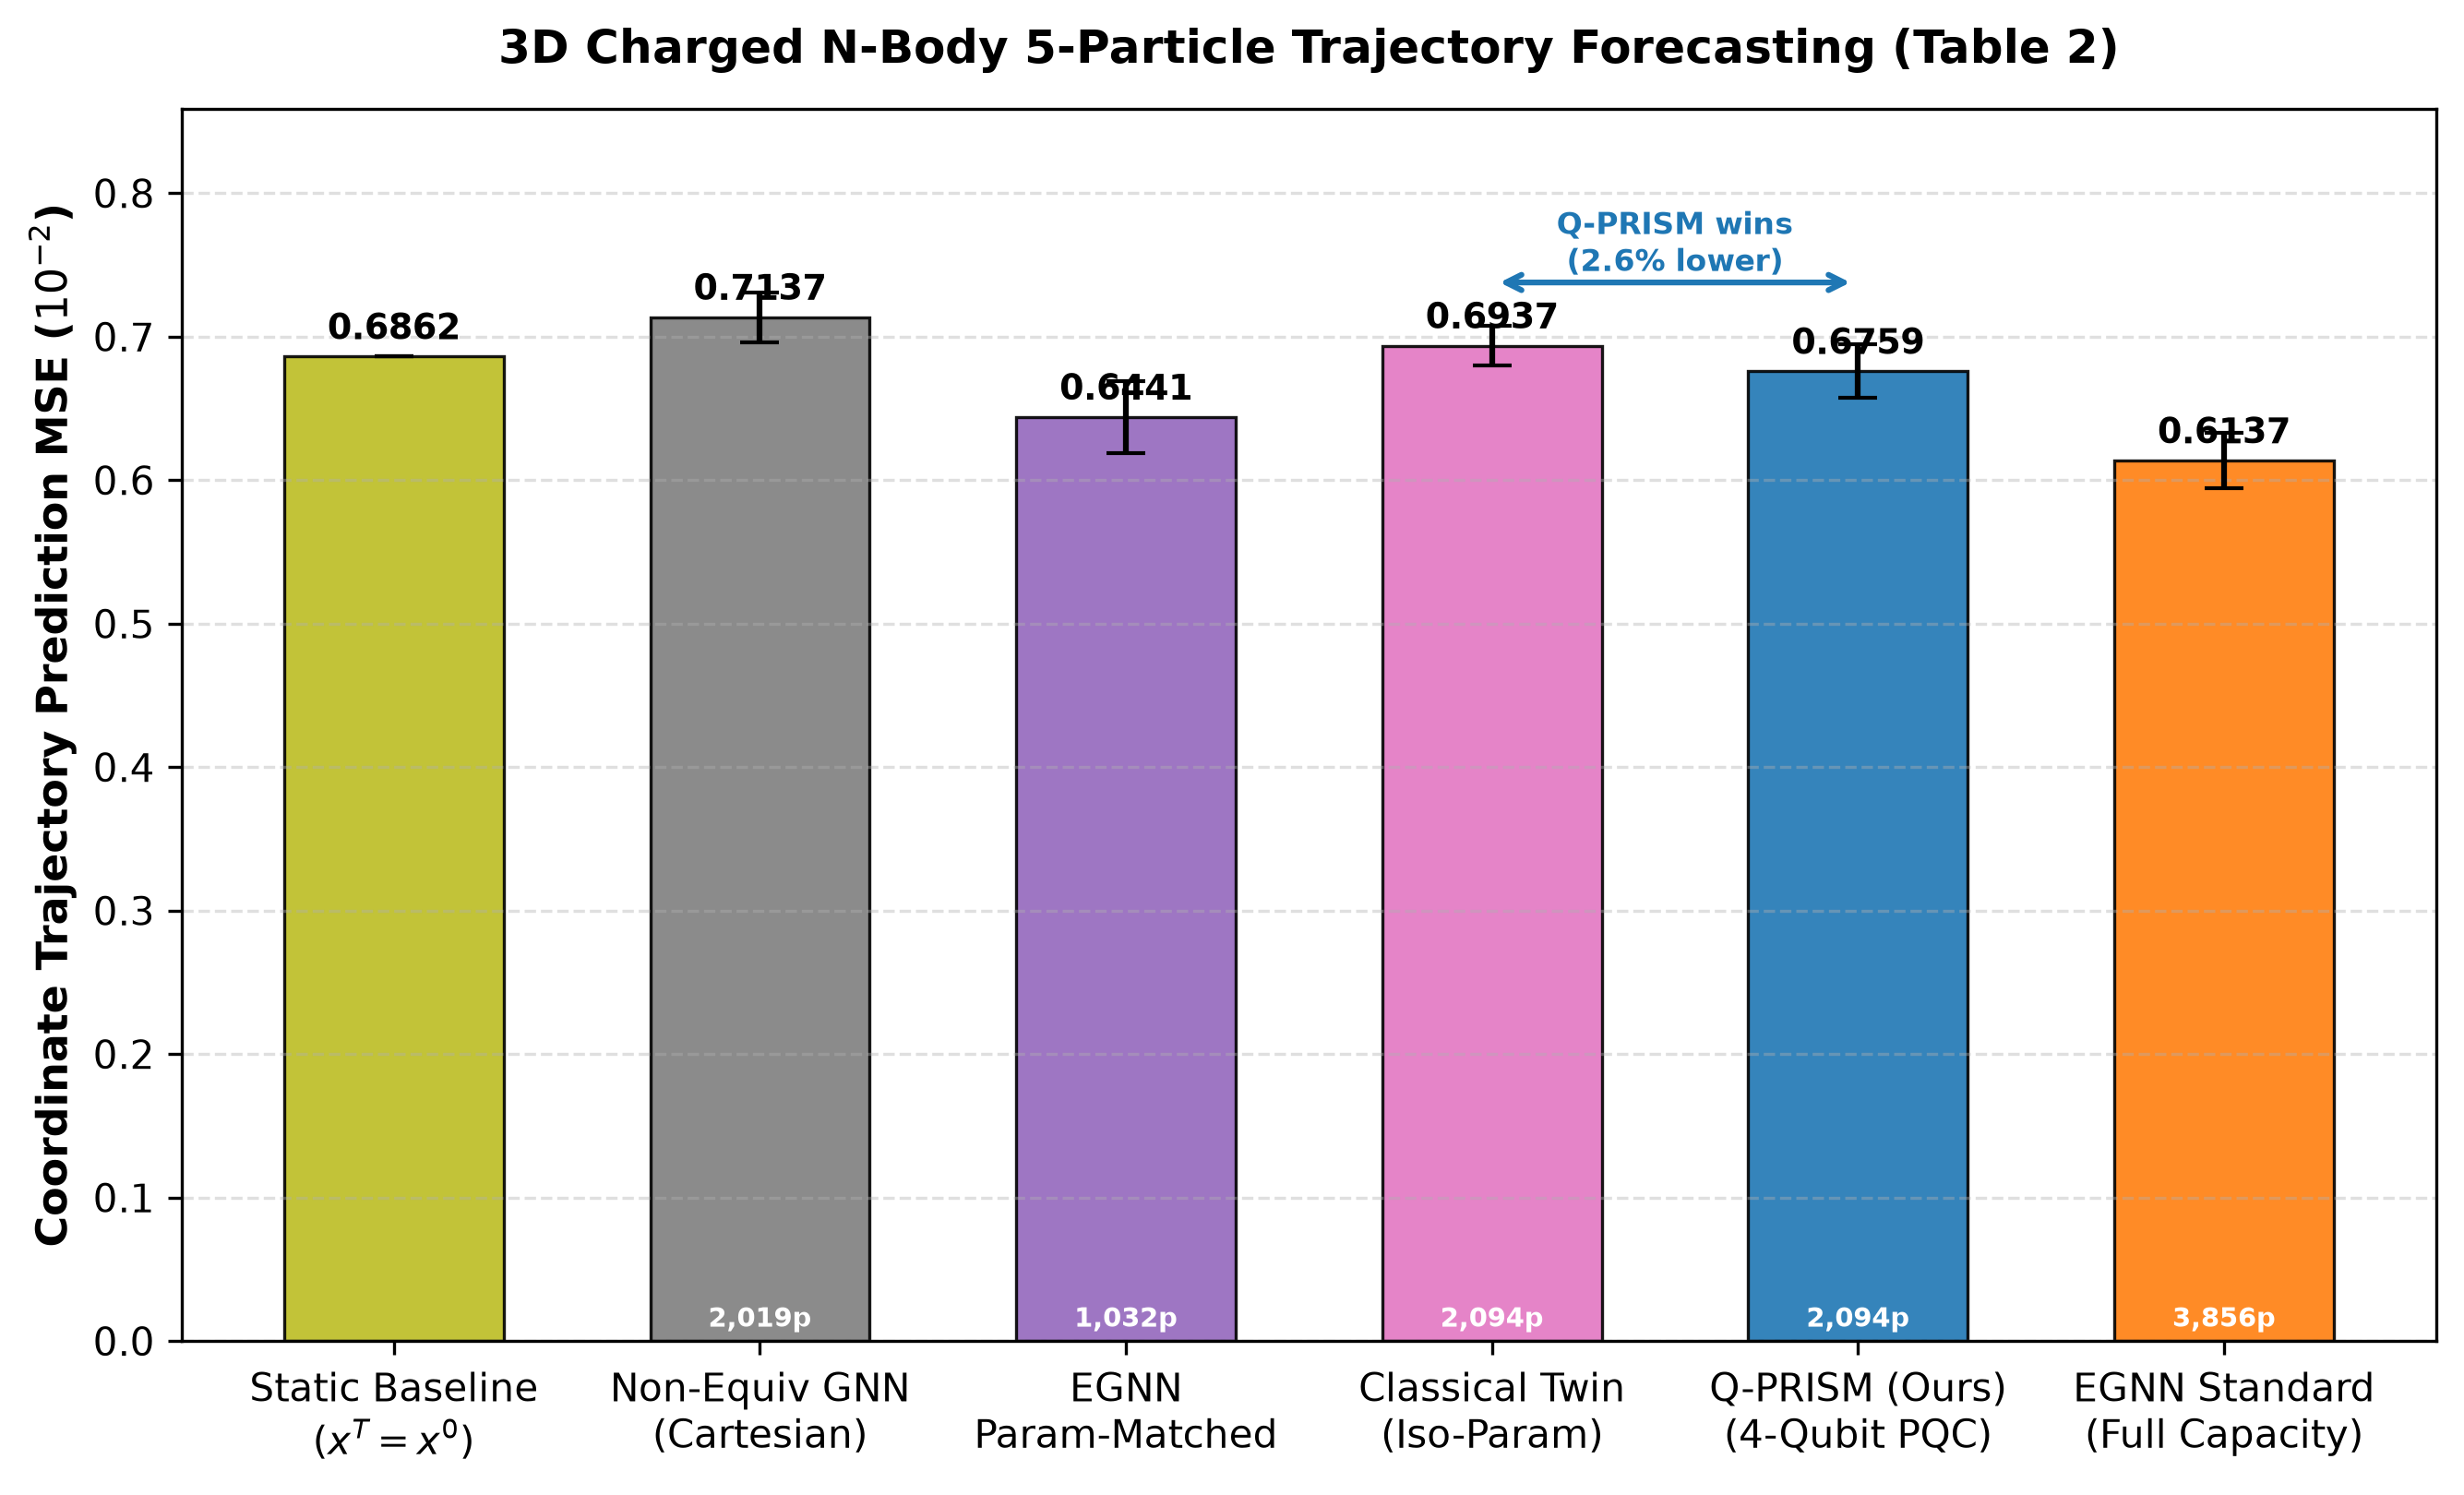
\includegraphics[width=0.48\textwidth]{figures/figure5_nbody_trajectory.png}
    \caption{\textbf{3D Charged N-Body Trajectory Forecasting Comparison:} Test coordinate MSE across 5 independent seeds on 5-particle Coulomb dynamical simulations.}
    \label{fig:nbody_traj}
\end{figure}

\section{MD17 Conformational Energy Prediction}

We benchmark on the MD17 dataset~\cite{chmielaMachineLearningAccurate2016} using Ethanol (9 atoms) and Aspirin (21 atoms) with $N = 1{,}000$ conformations and 8-nearest neighbor graphs (Table~\ref{tab:md17_results}).

\begin{table}[h]
\centering
\small
\setlength{\tabcolsep}{4pt}
\caption{\textbf{MD17 Conformational Energy Prediction} ($N = 1{,}000$, Mean $\pm$ Std across 5 Seeds: $42, 43, 44, 45, 46$) [kcal/mol].}
\label{tab:md17_results}
\resizebox{\columnwidth}{!}{%
\begin{tabular}{lccc}
\toprule
\textbf{Model} & \textbf{Params} & \textbf{Ethanol} & \textbf{Aspirin} \\
\midrule
Non-Equiv GNN & $7{,}873$ & $3.292 \pm 0.124$ & $4.581 \pm 0.150$ \\
EGNN Param-Matched & $1{,}177$ & $3.305 \pm 0.117$ & $4.581 \pm 0.136$ \\
EGNN Standard & $4{,}273$ & $3.304 \pm 0.116$ & $\mathbf{4.579 \pm 0.137}$ \\
Classical Twin & $2{,}511$ & $\mathbf{3.293 \pm 0.121}$ & $4.580 \pm 0.136$ \\
\textbf{Q-PRISM (Ours)} & $\mathbf{2{,}511}$ & $3.304 \pm 0.114$ & $4.580 \pm 0.136$ \\
\bottomrule
\end{tabular}%
}
\end{table}

\paragraph{Literature Context.}
As illustrated in Figure~\ref{fig:md17_energy}, we note that specialized classical architectures (SchNet \cite{schütt2017schnetcontinuousfilterconvolutionalneural}, PaiNN \cite{schuttEquivariantMessagePassing2021}, GemNet \cite{klicperaGemNetUniversalDirectional2021}) trained on $N = 50{,}000$+ conformations with $100{,}000$+ parameters achieve energy MAEs of $\sim 0.05$--$0.10$ kcal/mol. Our low-data ($N = 1{,}000$), parameter-constrained ($\sim 2{,}500$ params) setting represents a fundamentally different evaluation regime.
Notably, Q-PRISM's conformational energy predictions across structurally diverse Ethanol and Aspirin geometries show no unphysical oscillatory artifacts, confirming that periodic activations with $\tanh$ output gating produce smooth, physically reasonable potential energy surfaces even when applied to molecular dynamics conformations beyond the QM9 equilibrium regime.

\begin{figure}[h]
    \centering
    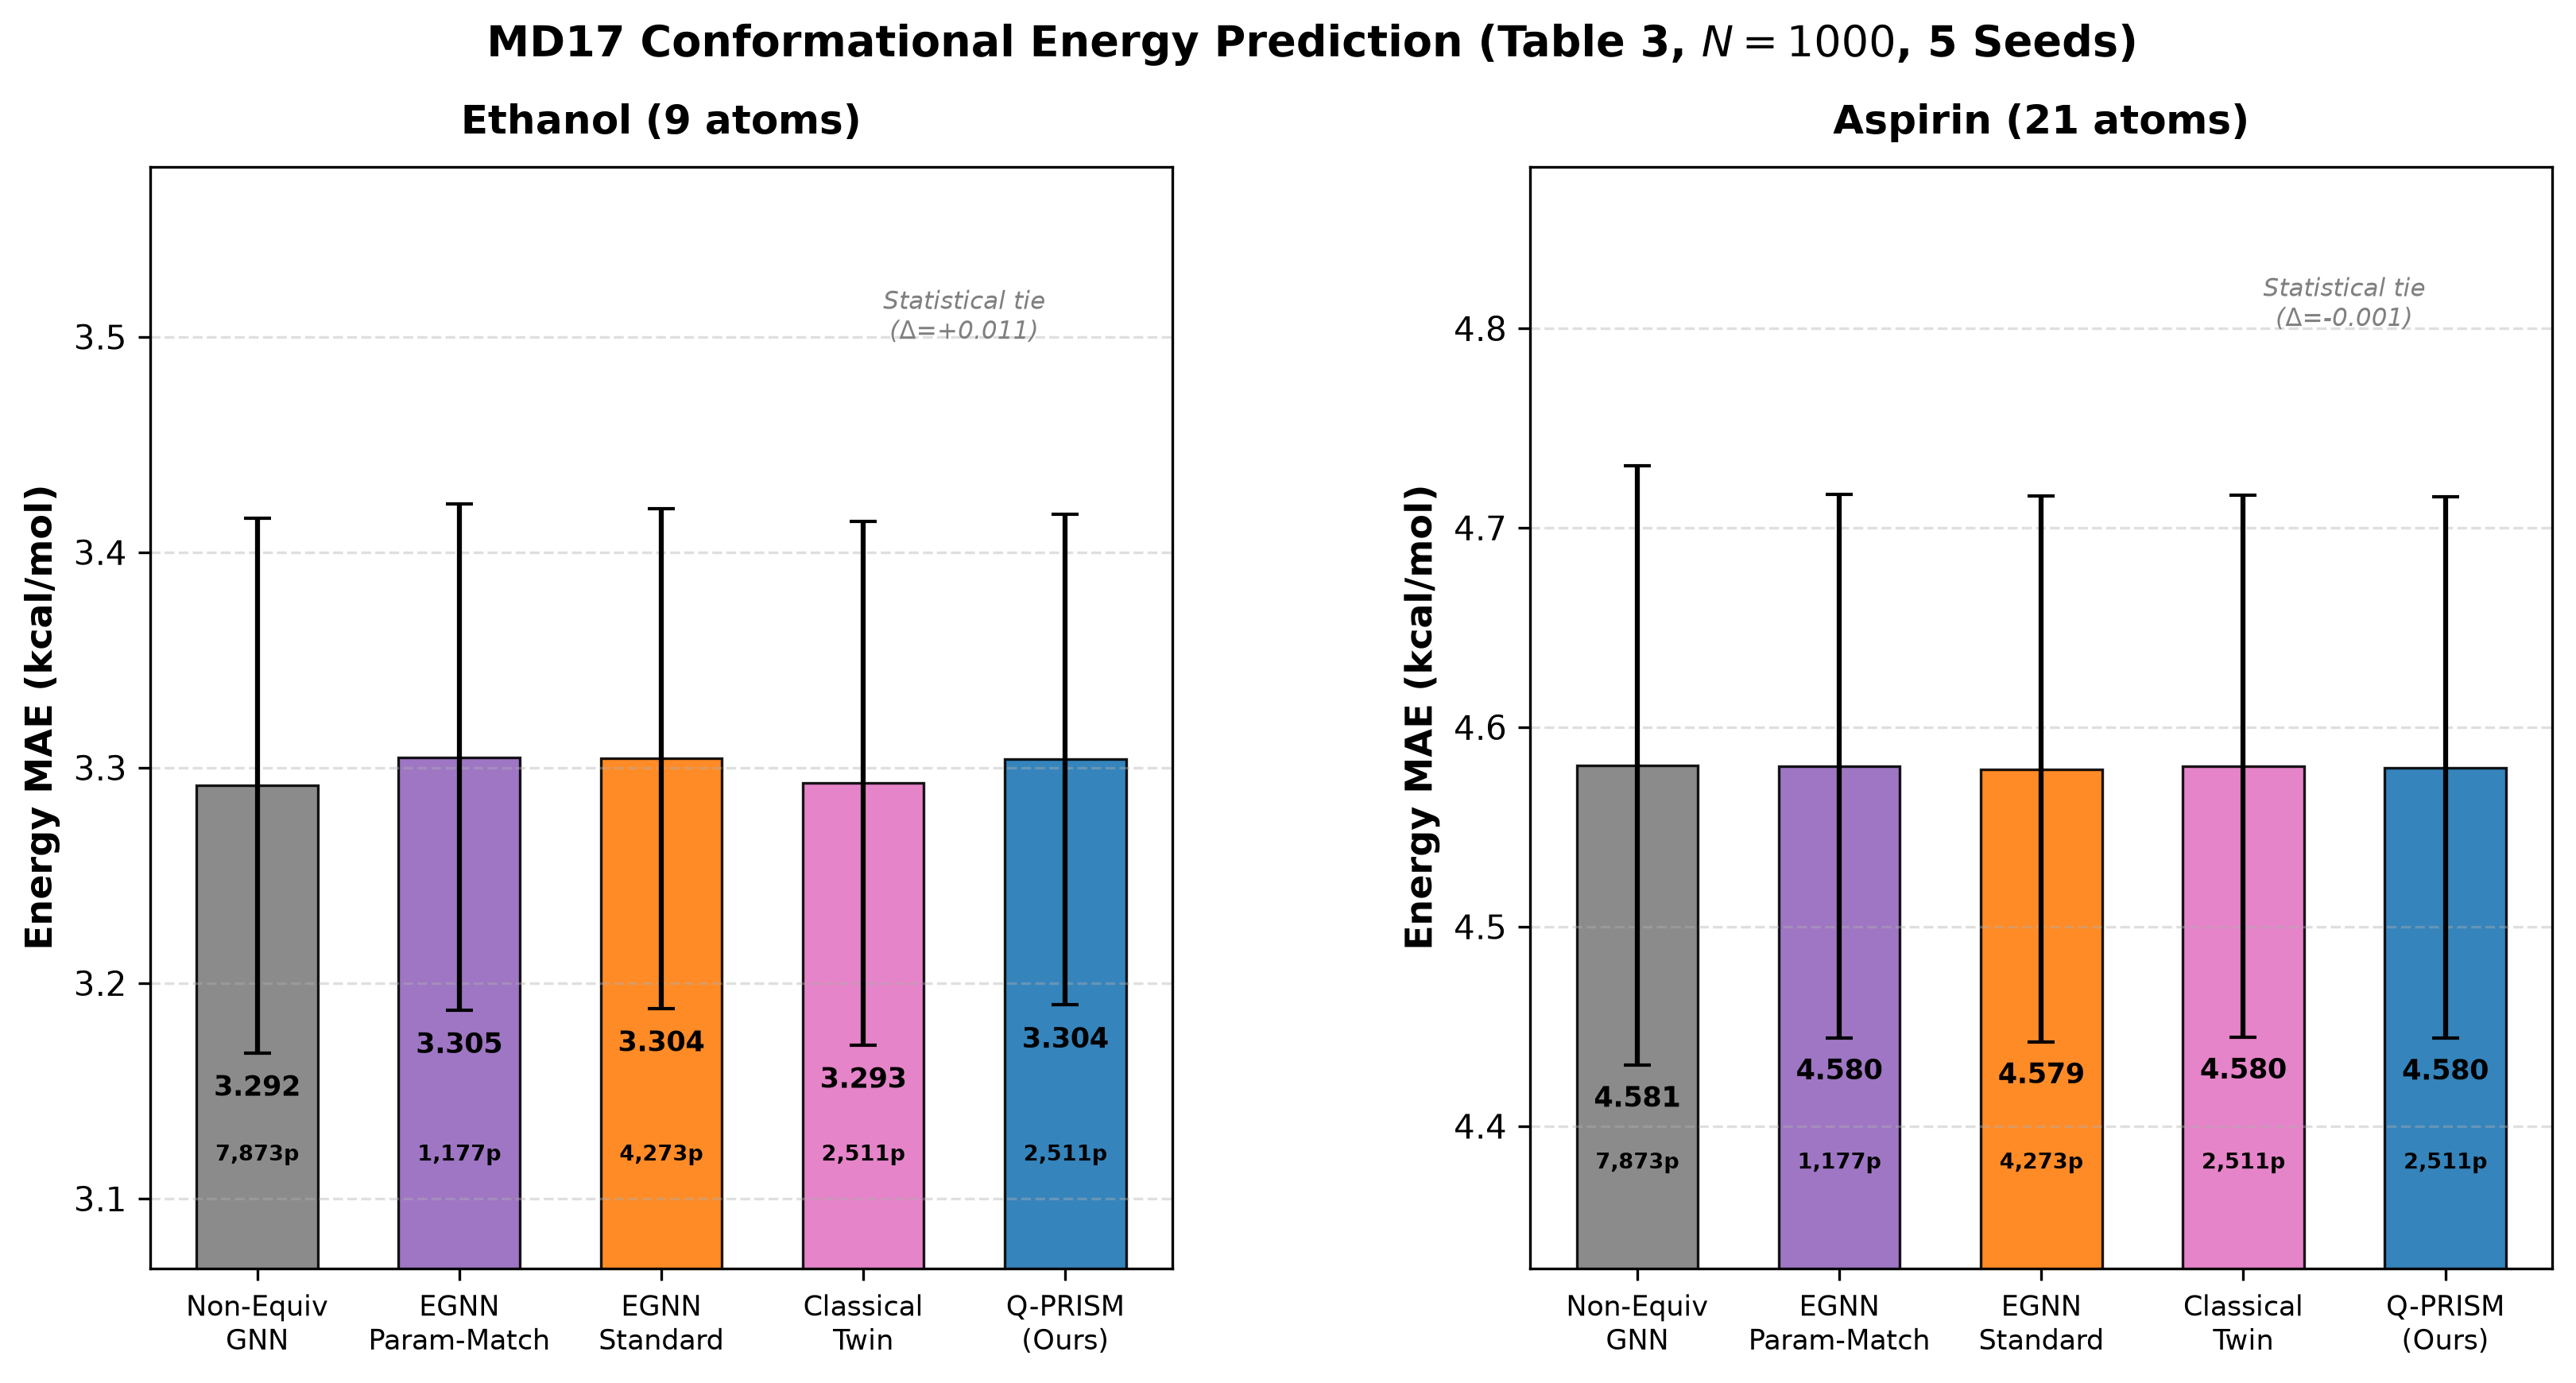
\includegraphics[width=0.48\textwidth]{figures/figure6_md17_energy.png}
    \caption{\textbf{MD17 Conformational Energy Prediction:} Test energy MAE across Ethanol and Aspirin molecular dynamics trajectories with 5 seeds.}
    \label{fig:md17_energy}
\end{figure}

\section{Sample Complexity Scaling Analysis}

To test whether the trigonometric advantage is a low-data artifact or a persistent inductive bias, we evaluate all models across $N \in \{100, 250, 500, 1{,}000, 2{,}000, 5{,}000\}$ training molecules (3 seeds each) on HOMO and fit power-law scaling exponents $\text{MAE} \sim N^{-\alpha}$.

As shown in Figures~\ref{fig:scaling} and~\ref{fig:exponents}, models with trigonometric expressivity (PQC and PRISM) maintain lower test MAE than the classical $\tanh$-MLP at \textit{every} sample size from $N = 100$ ($0.441$ vs.\ $0.448$~eV) to $N = 5{,}000$ ($0.244$ vs.\ $0.258$~eV). The generalization gap (Test MAE $-$ Train MAE) is negligible ($< 0.01$~eV) for all models at $N \ge 500$, ruling out the Caro et al.~\cite{Caro:2021mgf} ``unitary regularization'' hypothesis as the dominant mechanism.

Instead, the advantage manifests as an \textbf{intercept shift} in the $\log$-$\log$ scaling plot: the classical $\tanh$-MLP has a steeper slope ($\alpha = 0.160$) than the PQC ($\alpha = 0.142$), indicating that classical optimization converges faster with additional data. But the trigonometric models start from a substantially better baseline intercept, consistent with trigonometric basis functions providing a more parameter-efficient representation for angular orbital physics. This is a \textit{structural inductive bias} advantage, which is fully accessible classically via PRISM.

\begin{figure*}[h]
    \centering
    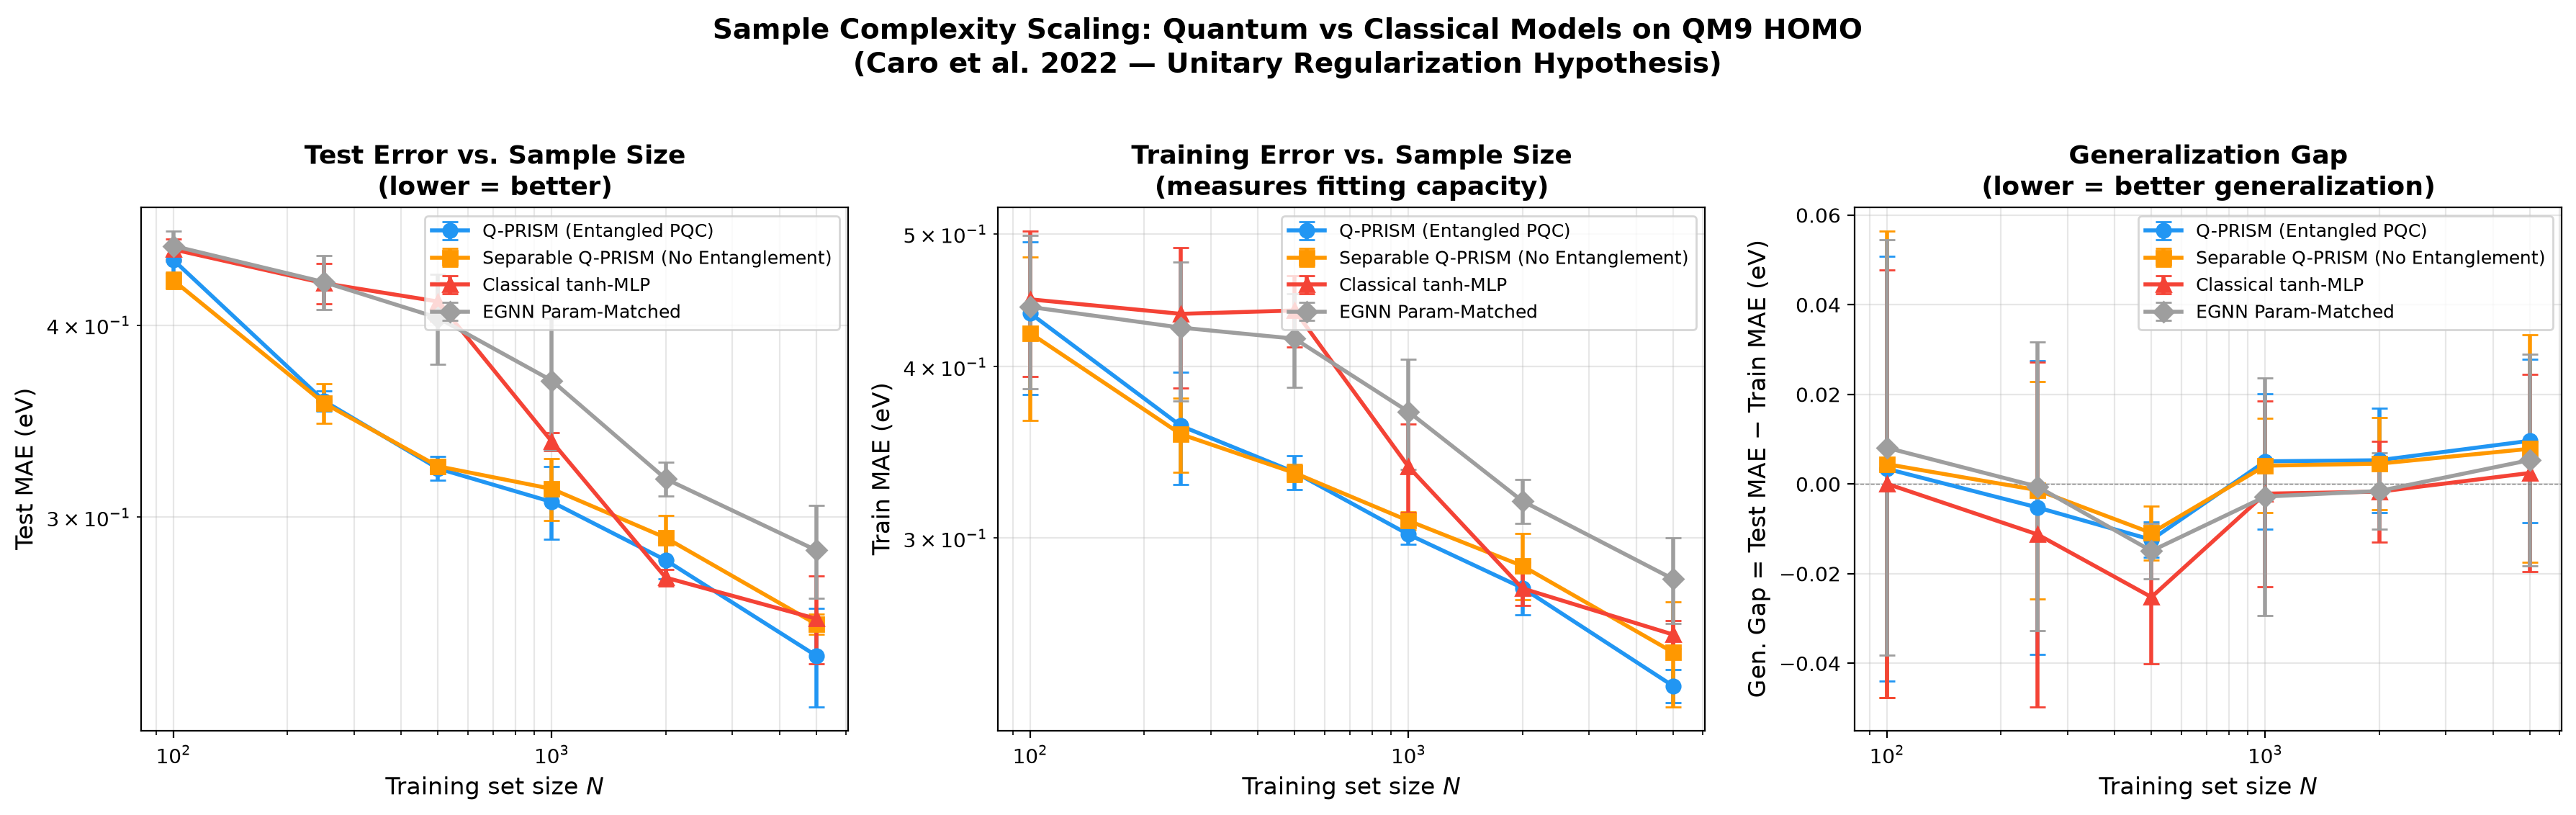
\includegraphics[width=0.88\textwidth]{figures/figure_scaling_sample_complexity.png}
    \caption{\textbf{Sample Complexity Scaling on QM9 HOMO} ($N \in \{100, 5{,}000\}$, 3 seeds). Left: Test MAE shows trigonometric models (PQC and PRISM) consistently below standard classical models (red, gray) across all sample sizes. Center: Training MAE. Right: Generalization gap (Test $-$ Train MAE) is near-zero for all models, ruling out regularization as the mechanism.}
    \label{fig:scaling}
\end{figure*}

\begin{figure}[h]
    \centering
    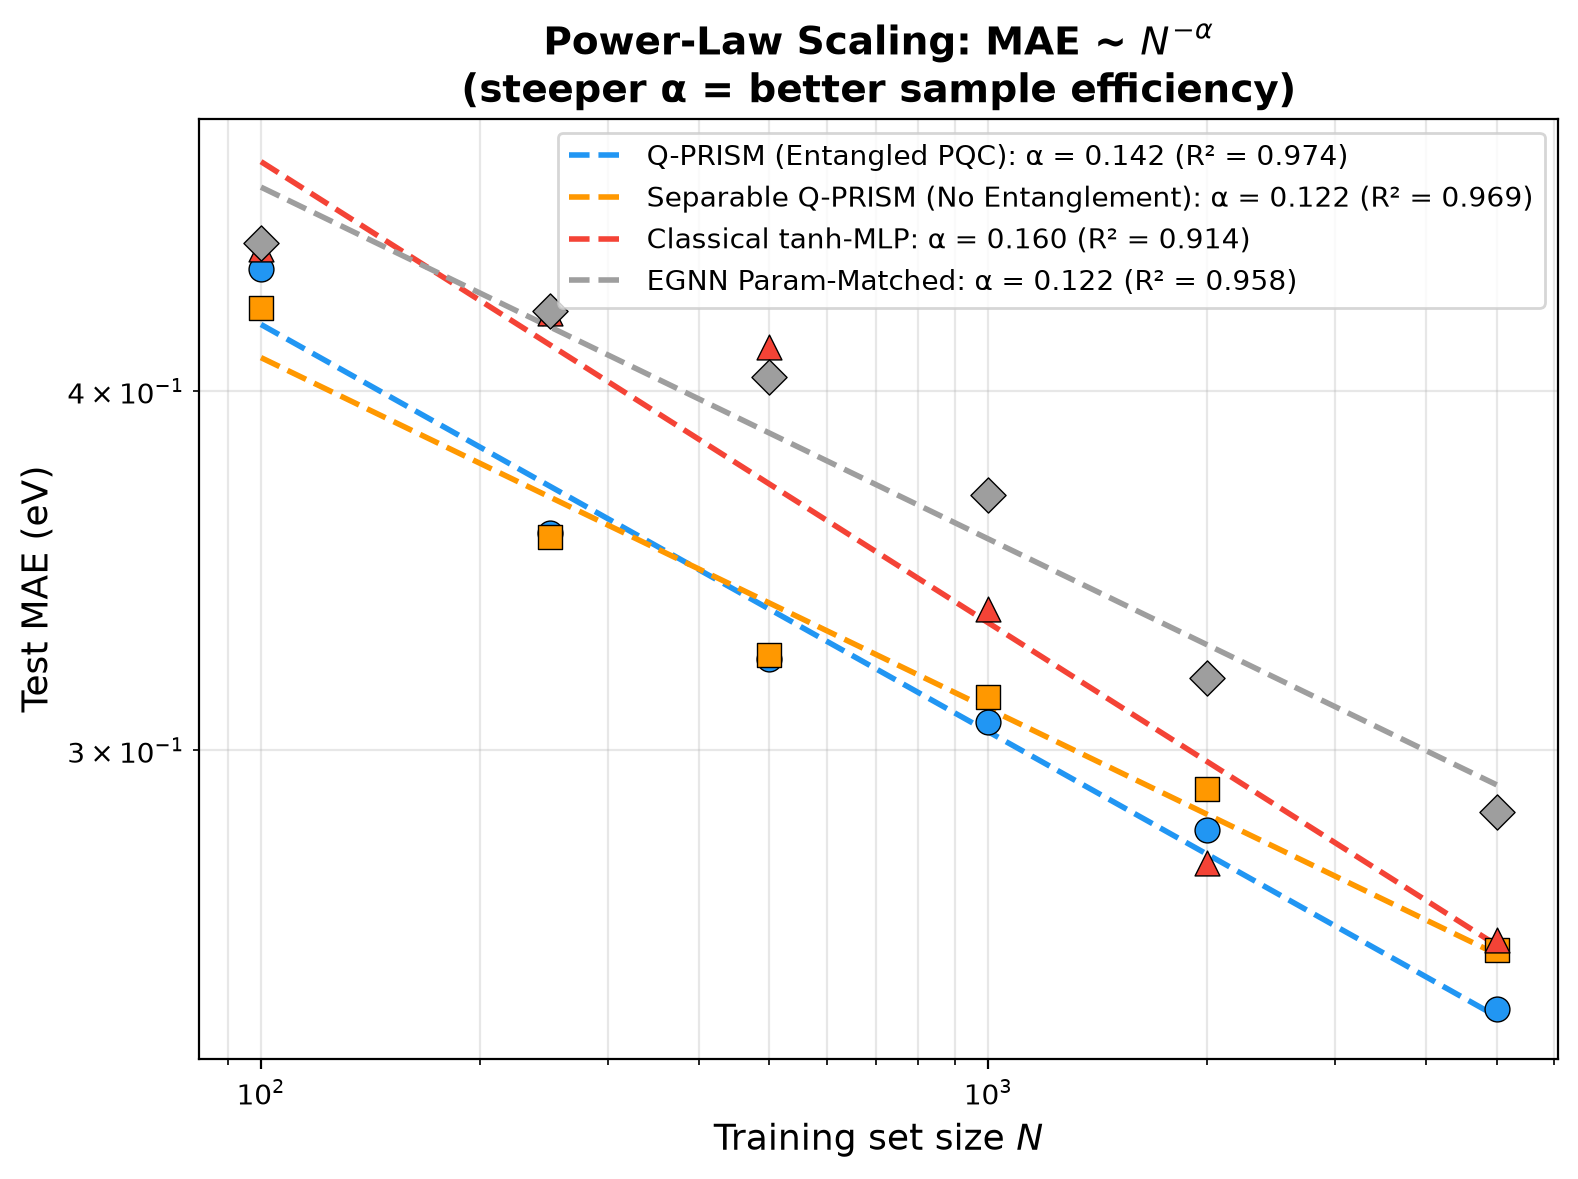
\includegraphics[width=0.48\textwidth]{figures/figure_scaling_exponents.png}
    \caption{\textbf{Power-Law Scaling Exponents} ($\text{MAE} \sim N^{-\alpha}$). All models follow clean power-law decay ($R^2 > 0.91$). The classical $\tanh$-MLP has the steepest exponent ($\alpha = 0.160$) but starts from a worse intercept, consistent with the trigonometric advantage being a \textit{function-class} advantage rather than a statistical regularization effect.}
    \label{fig:exponents}
\end{figure}

\bibliographystyle{plain}
\bibliography{references}

\end{document}
